\documentclass[12pt,a4paper,oneside]{report}
\usepackage{pdfpages}
\usepackage[utf8]{inputenc}
\usepackage[T1]{fontenc}
\usepackage[margin=2.5cm]{geometry}
\usepackage{graphicx}
\usepackage{amsmath,amssymb}
\usepackage{booktabs}          
\usepackage{tabularx}
\usepackage{listings}          
\usepackage{xcolor}
\usepackage{caption}
\usepackage{subcaption}
\usepackage{setspace}
\usepackage{float}
\usepackage[toc,page,title,titletoc]{appendix}
\renewcommand{\appendixpagename}{Appendices}
\renewcommand{\appendixtocname}{Appendices}
\usepackage{enumitem}
\usepackage[backend=biber,style=authoryear,sorting=nyt,maxcitenames=3,mincitenames=1,maxbibnames=99]{biblatex}
\renewcommand*{\nameyeardelim}{\addcomma\space}
\DefineBibliographyStrings{english}{
  bibliography = {References},
}


\defbibenvironment{bibliography}
  {\enumerate[label={[\arabic*]},leftmargin=*,labelsep=1ex,itemsep=0.4\baselineskip]}
  {\endenumerate}
  {\item}

\addbibresource{references.bib}

%---------------------------------------------------------------- code style
\definecolor{codegray}{gray}{0.95}
\definecolor{commentgreen}{rgb}{0.0,0.5,0.0}
\definecolor{keywordblue}{rgb}{0.0,0.0,0.7}
\lstdefinestyle{csharp}{
  language=[Sharp]C,
  backgroundcolor=\color{codegray},
  basicstyle=\ttfamily\footnotesize,
  keywordstyle=\color{keywordblue},
  commentstyle=\color{commentgreen}\itshape,
  numbers=left, numberstyle=\tiny, numbersep=6pt,
  breaklines=true, showstringspaces=false, frame=single, tabsize=2
}
\lstset{style=csharp}

\definecolor{stringred}{rgb}{0.63,0.13,0.13}
\lstdefinestyle{python}{
  language=Python,
  backgroundcolor=\color{codegray},
  basicstyle=\ttfamily\footnotesize,
  keywordstyle=\color{keywordblue},
  commentstyle=\color{commentgreen}\itshape,
  stringstyle=\color{stringred},
  numbers=left, numberstyle=\tiny, numbersep=6pt,
  breaklines=true, showstringspaces=false, frame=single, tabsize=4, captionpos=b
}

\onehalfspacing

%============================================================================
%  COVER
%============================================================================
\begin{document}

\begin{titlepage}
    \centering

    % Title centred vertically
    \vspace*{\fill}

    {\Large\bfseries
    Adaptive Difficulty Through Bayesian Opponent Modelling\\[0.35cm]
    in ISMCTS-Based Card Game Agents\par}

    \vspace*{\fill}

   
    \begin{flushleft}
        \begin{tabular}{@{}ll}
            \textbf{Author:} & José Pablo González Poblette \\[0.2cm]
            \textbf{Student ID:} & 2507739 \\[0.2cm]
            \textbf{Degree:} & Master of Science in Computer Games Technology \\[0.2cm]
            \textbf{Faculty:} & Faculty of Design, Informatics and Business \\
            & Abertay University \\[0.2cm]
            \textbf{Date:} & August 2026
        \end{tabular}
    \end{flushleft}

    \vspace{1.2cm}

\end{titlepage}

\pagenumbering{roman}

% ---- Abstract ----
\chapter*{Abstract}
\addcontentsline{toc}{chapter}{Abstract}

 Information Set Monte Carlo Tree Search (ISMCTS) is a version of Monte Carlo Tree Search (MCTS) designed to handle games with hidden information. This dissertation expands on this approach by replacing its standard uniform sampling of hidden states with an adaptive, belief-driven alternative based on Bayes’ theorem. Instead of assigning equal probability to each possible hidden state, the proposed method incorporates the observable evidence revealed by the actions of an opponent to bias the determinization towards the hidden states that their observed play makes more reasonable. The study investigates whether this Bayesian approach affects the performance of the ISMCTS agent and how real players perceive the resulting opponent.

The approach will be implemented and evaluated using the card game Cambio. The proposed agent will be tested in two ways: first, against a baseline ISMCTS agent, and second, through playtesting with human participants to support more objective conclusions about its performance and player experience.

\vspace{3em}
\noindent\textbf{Keywords:} Information Set Monte Carlo Tree Search (ISMCTS), Bayesian inference, opponent modelling, Determinization, imperfect-information games, dynamic difficulty adjustment, player perception, Cambio.
\tableofcontents


\listoffigures
\addcontentsline{toc}{chapter}{List of Figures}

\listoftables
\addcontentsline{toc}{chapter}{List of Tables}

\clearpage
\pagenumbering{arabic}


%  CHAPTER 1 -- INTRODUCTION
%============================================================================
\chapter{Introduction}
\label{ch:intro}
\section{Background and Motivation}

Artificial intelligence is widely used in video games, where one of its main purposes is to provide players with opponents to interact with and compete against. Early implementations, such as the ghost behaviours in Pac-Man, demonstrate how AI can enhance the player experience and create engaging gameplay. However, one challenge for game AI is predictability, as players become familiar with its behaviours over time. As the complexity of a game increases, the AI must also process a greater amount of information and consider a larger number of possible decisions, making it increasingly difficult to maintain challenging and engaging opponents.

Many algorithms have been developed to address this problem. Monte Carlo Tree Search (MCTS) uses a method for constructing a search tree by repeatedly simulating possible future actions. MCTS has been particularly successful in perfect-information games such as chess or Go, where the complete game state is visible to all players at all times. However, many games do not provide players with complete information about the current state. Consequently, the AI must make decisions while inferring information about the hidden state. These games are generally refereed to as imperfect-information games. 

In a card game, for example, a player's hand may be hidden from their opponent, meaning that multiple possible game states are consistent with the information currently available to each player. This creates an additional layer of uncertainty that does not exist in a standard perfect-information game. An AI cannot simply determine the exact current state and search forward from it; instead, it must consider a set of possible states that could represent the actual game state.

This issue is particularly relevant to the card game Cambio, which is the game environment considered in this research. In Cambio, players have hidden cards and must make decisions without knowing the complete contents of their opponents' hands. However, players can obtain information about these hidden cards through the progression of the game. Cards that have already been revealed or discarded reduce the set of cards that could still be hidden, while actions such as swapping cards, using powers, or making other decisions can provide additional information about an opponent's possible hand. Therefore, the decisions made by a player can provide evidence about information that would otherwise remain hidden. This makes Cambio an appropriate environment for investigating whether an AI can use observations of player behaviour to adapt its representation of hidden information.

To address imperfect-information games, \textcite{cowling2012ismcts} introduced Information Set Monte Carlo Tree Search (ISMCTS), extending the principles of MCTS to situations in which the complete game state is not known.

A key component of ISMCTS is the use of determinization. Before a simulation, the unknown parts of the game state are assigned values to produce one possible complete game state, after which the simulation can proceed using the principles of standard MCTS. In a conventional implementation, these determinizations are sampled uniformly from the states that are consistent with the information currently available to the player. In other words, if several possible hidden configurations exist, each is treated as equally likely when selecting a determinization.

Although this approach allows ISMCTS to perform fine in an imperfect-information environment, treating every consistent hidden state as equally probable is not necessarily representative of how uncertainty occurs during actual gameplay. In a card game, the information available to a player changes continuously as cards are revealed, discarded, swapped, or otherwise affected by player actions. Similarly, an opponent's behaviour may provide additional evidence about the hidden state. For example, in Cambio, the cards an opponent chooses to exchange, the way they use available powers, and the actions they choose to take may provide information about the cards they are likely to hold. Two hidden states that are both technically possible may not be equally plausible given the evidence observed during the game.

This motivates the use of a belief over possible hidden states rather than treating all possible determinizations uniformly. A belief distribution can assign different probabilities to different hidden states according to the evidence available at a particular point in the game. As additional evidence is observed, these probabilities can be updated, allowing the representation of hidden information to adapt throughout the game.

Bayes' theorem provides a mathematical foundation for updating such beliefs when new evidence becomes available.

The ability to adapt to opponents is particularly relevant when developing efficient and engaging game AI. Many card games rely heavily on interaction between multiple players, and the quality of the opponents can have a significant influence on the overall player experience. A static AI may provide an effective challenge initially but can become predictable once players understand its decision-making patterns. Developing AI models that approach games in different ways may provide a way to create opponents that remain more engaging as players become familiar with them. At the same time, the computational efficiency of the approach remains important, since an AI must make decisions within the time and computational constraints of an interactive game.

This research therefore proposes the integration of an adaptive Bayesian layer with a standard ISMCTS agent. Rather than replacing ISMCTS, the proposed approach aims to modify the way the agent represents and samples uncertainty about hidden information. The Bayesian component can update beliefs about possible hidden states as evidence is observed throughout the game, while opponent modelling can be used separately to represent beliefs about the behaviour or strategy of the opponent. These beliefs can then inform the determinization process used by ISMCTS.

The research investigates whether integrating these ideas into an adaptive layer can produce a meaningful difference in the perceived quality and difficulty of an AI opponent in the card game Cambio.   


\section{Aim and Objectives}

The objectives can be divided into three main categories:
\begin{enumerate}
    \item Create a belief-weighted sampler to use in ISMCTS based on Bayes' theorem.
    \item Test standard ISMCTS against my take on it, running them against each other and against actual human players.
    \item Compare the AIs' results with two metrics: an objective one that validates their score and win rate, and a qualitative one gathered via a form given to the play testers.
\end{enumerate}

The aim is to see whether adding this layer provides any value to the current ISMCTS or is not necessary. It could add value in the way of player perception, or as an objectively better model for this short game.

\section{Research Question}

Does integrating an adaptive Bayesian opponent-modelling layer into a static ISMCTS agent influence player-perceived opponent quality and difficulty in a card game compared to a static ISMCTS?

\section{Scope and Limitations}

This research expands the ISMCTS framework by adding an adaptive Bayesian layer that supplies dynamically updated beliefs to shape the determinizations of the underlying search responsible for decision-making. The goal is not optimal play or convergence to a Nash equilibrium. Since the agent acts on probabilistic beliefs rather than complete knowledge, its decisions will sometimes be effective and sometimes mistaken. This is an intentional design decision, as the research investigates whether an agent that adapts its beliefs to observed behaviour produces a more organic and less predictable opponent, rather than a stronger one.

Several factors limit the generalisability of the results. Cambio was chosen precisely because its small set of variables and actions makes the approach feasible to build and evaluate in the time available, and lets the study isolate the interaction between ISMCTS, Bayesian belief updating, and opponent modelling. That same simplicity limits generalisability: behaviour in Cambio may not carry over to games with larger state and action spaces or more sophisticated opponents.

The three-month development period is a further constraint, restricting how polished the interface can be and leaving the game reliant in part on text-based feedback. If the agent's adaptation is not clearly conveyed, players may not perceive it, so a lack of difference in perceived opponent quality would not necessarily mean the belief layer failed to adapt internally, only that the adaptation was not visible. Finally, the sample consists of 20 participants across 400 games, which limits statistical power and generalisability. The findings should therefore be interpreted within the context of this specific game, implementation, and participant group. 

\section{Dissertation Structure}

This dissertation is organised as follows. Chapter~\ref{chap:litreview}
reviews the relevant literature, covering imperfect-information games and belief modelling,
the family of search-based methods that leads to ISMCTS, counterfactual regret
minimisation, Bayesian inference, and dynamic difficulty adjustment.  It then identifies the gap this work addresses. Chapter~\ref{chap:methodology} sets out the research approach,
formalises the card game Cambio as the experimental environment, describes the system
architecture, and defines the evaluation methodology, including the user study design and
the behavioural and computational metrics used to answer the research question.

Chapter~\ref{chap:design} details the design and implementation of the system. It describes
the game core and its single mutation path, the card model and scoring, the determinization
support used by the search, and the ISMCTS agent itself, before presenting the Bayesian
belief layer, the adaptive opponent-modelling layer, and the mechanisms introduced to keep
the agent unpredictable. Chapter~\ref{chap:results} reports the results of the evaluation
across three strands: computational performance, the user study, and an analysis of the
behavioural weights learned during play. Chapter~\ref{chap:discussion} interprets these
results in relation to the research question and situates them against the reviewed
literature. Chapter~\ref{chap:conclusion} concludes the dissertation and outlines directions
for future work, including how the approach could be extended beyond the constraints of the
current study. The questionnaire administered to participants is reproduced in
Appendix~\ref{app:questionnaire}.


%  CHAPTER 2 -- LITERATURE REVIEW / BACKGROUND

\chapter{Literature Review}\label{chap:litreview}
\label{ch:litreview}

This chapter reviews the work on which this dissertation builds. It begins by introducing imperfect-information games and the representation of hidden states through beliefs. It then traces the development of search-based methods leading to ISMCTS and contrasts these with counterfactual regret minimisation as an equilibrium-based alternative. Finally, it examines Bayesian inference as the foundation for updating beliefs and identifies the research gap addressed by this work.


\section{Imperfect-Information Games and Belief Modelling}

Chapter~\ref{ch:intro} introduced imperfect-information games as games in which part of the state is hidden, meaning that a player can identify only the set of states consistent with their observations rather than the single true state. This section examines how an agent can represent this uncertainty. A natural approach is to maintain a belief, which is a probability distribution over the possible hidden states. Each state is assigned a probability according to how well it agrees with the evidence observed so far, and these probabilities are revised as further evidence becomes available \parencite{frank1998search}. Rather than committing to a single guess about the hidden state, the agent maintains a graded estimate that can become more precise or change as the game progresses.

This is different from opponent modelling. A hidden-state belief represents uncertainty about the underlying game state, such as the cards an opponent may hold. An opponent model by contrast represents beliefs about how an opponent behaves or makes decisions. The two concepts can be related because an opponent's behaviour can provide evidence that changes the probability assigned to different hidden states. This relationship is where the present work is situated. The agent assumes a fixed model of rational opponent behaviour and uses observed actions as evidence to update its belief about the opponent's hidden cards. It does not learn or adapt its model of the opponent's strategy itself. The opponent model therefore acts as a mechanism for hidden-state inference rather than as a broader model of opponent behaviour of the kind described by, for example, \textcite{southey2005bayes}.

\section{Search-Based Methods in Game AI}

\subsection{Monte Carlo Tree Search}

Monte Carlo Tree Search (MCTS) is a best-first search algorithm that builds an
asymmetric tree incrementally by running many simulated playouts rather than
exhaustively evaluating a fixed-depth frontier \parencite{coulom2006efficient}. Each
iteration consists of four phases: selection, expansion, simulation, backpropagation.

First in selection, the algorithm descends from the root through already-expanded nodes according to a tree policy until it reaches a node with unexpanded children. In expansion, one such child is added to the tree. In simulation, a playout is run from the new node to a terminal state using a default random policy, producing an outcome. Finally in backpropagation, that outcome is propagated back along the visited path, updating the visit count and accumulated value of every node on it. Over many iterations, the tree grows deeper in regions that repeated simulations suggest are promising, so the search effort is concentrated where it is most likely to matter.

The tree policy governs the balance between exploring under-sampled moves and
exploiting moves that have performed well so far. The standard choice is the Upper
Confidence Bound applied to Trees (UCT), which treats the selection at each node as a
multi-armed bandit problem and selects the child maximising
$\bar{X}_j + C\sqrt{\ln n / n_j}$, where $\bar{X}_j$ is the mean outcome of child $j$,
$n$ and $n_j$ are the visit counts of the parent and child, and $C$ controls the
weight given to the exploration term \parencite{kocsis2006bandit}. This formulation gives
MCTS an anytime property and removes the need for a hand-crafted evaluation function,
which contributed to its success across a wide range of domains
\parencite{browne2012survey}. However, standard MCTS assumes that the state at the root is
fully known, since both the tree policy and the simulation phase operate on a single,
completely specified game state. In an imperfect-information game this assumption does
not hold, because the true state is not directly observable and many states are
consistent with what the player can see. This limitation is what Information Set MCTS,
described next, is designed to address.

\subsection{Information Set MCTS (ISMCTS)}

In imperfect-information games, an information set can be understood as a collection of game states that are indistinguishable to a player given the information available to them \parencite{cowling2012ismcts}. A player knows which information set they occupy, but cannot determine which specific state within that information set is the true state. ISMCTS modifies the structure of standard MCTS so that nodes represent information sets rather than individual game states. This allows information from simulations corresponding to multiple possible states to be collected within a common search tree, making more efficient use of the available computational budget.

% Example figure include (drop MCTS diagram into figures/):
\begin{figure}[h]\centering
   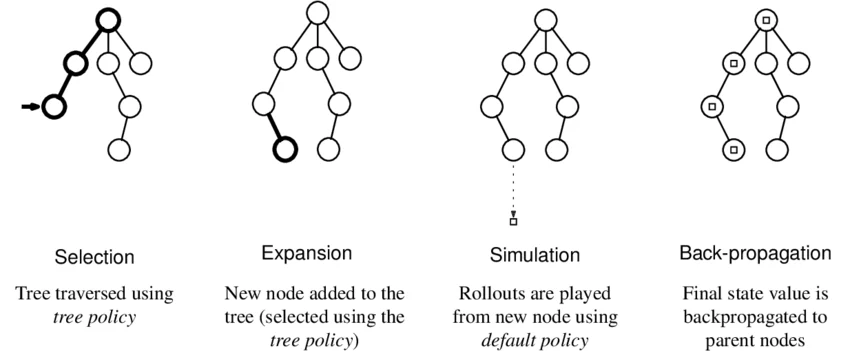
\includegraphics[width=0.9\textwidth]{images/mcts_diagram.png}
   \caption{The four MCTS phases: selection, expansion, simulation,backpropagation.}
   \label{fig:mcts}
\end{figure}

\section{Counterfactual Regret Minimization}

Counterfactual Regret Minimisation (CFR) approaches imperfect-information games
from a different direction than the search-based methods described above. Rather
than building a search tree forward from the current state, CFR is an iterative
self-play algorithm that repeatedly plays the entire game against itself and
refines a strategy at every information set. On each iteration it records, for
each action available at an information set, a measure of \emph{regret}: how much
better the player would have done, in retrospect, had it always chosen that action
rather than the strategy it actually followed. Actions are then reweighted in
proportion to their accumulated positive regret, so that choices which would have
paid off are played more often in subsequent iterations. A central result is that
although the strategy on any single iteration may be poor, the \emph{average}
strategy over many iterations converges towards a Nash equilibrium
\parencite{zinkevich2007regret}.

A Nash equilibrium is a profile of strategies in which no player can improve their
expected outcome by unilaterally changing their own strategy. In two-player
zero-sum games this corresponds to an unexploitable strategy: one that guarantees a
bounded loss against any opponent, however that opponent chooses to play. This
property has made CFR and its successors the foundation of the strongest computer
poker agents. Brown and Sandholm's~(\citeyear{brown2019superhuman}) Pluribus, built on these
ideas, was able to defeat professional human players at multiplayer no-limit Texas
hold'em, a landmark result for imperfect-information game AI.

However, the objective that makes CFR powerful is also what limits its relevance to
this project. CFR is designed to approximate an equilibrium, and an equilibrium
strategy is by definition one that does not depend on the specific opponent it
faces: it aims to be difficult to beat against every possible opponent rather than
to exploit the tendencies of any particular one. Such a strategy is also
essentially static once it has been computed, and computing it can be expensive,
typically requiring a very large number of self-play iterations over the game's
information sets. The goal of this research is not an unexploitable opponent but an
adaptive and believable one --- an agent that responds to how a specific human is
playing and remains engaging rather than mathematically optimal. CFR therefore provides a useful conceptual contrast: it defines what optimal play means in an imperfect-information game, while showing why optimality is not the same as adaptivity and why an equilibrium solver is not an appropriate basis for the opponent this project aims to build.

Accordingly, counterfactual regret minimisation is reviewed here for the
perspective it provides on optimality in imperfect-information games rather than
as a technique this dissertation implements; equilibrium solving falls outside the
scope of this work, and is included as one of several approaches surveyed in order
to situate the design that follows.




\section{Opponent Modelling and Believable Agents}
\label{sec:opponent-modelling}

The methods described so far aim to achieve strong play. The objective of opponent modelling is for an agent to observe the particular opponent it faces and adapt its behaviour accordingly, rather than attempting to play well against every possible adversary. \textcite{bakkes2009opponent} use case-based opponent models to support adaptive game AI, retrieving behaviour that has previously performed well against similar opponents and applying it to the current one. In imperfect-information games, opponent modelling and hidden-state inference can overlap because an opponent's observable actions may provide evidence about information that would otherwise remain hidden. Southey et al.'s~(\citeyear{southey2005bayes}) Bayesian treatment of poker, discussed further in the next section, provides a representative example.

A related body of work questions whether the strongest possible opponent is necessarily the most desirable. \textcite{arrabales2009conscious} argue for agents whose behaviour appears reasoned and human-like rather than strictly optimal, while \textcite{soni2008bots} found that bots trained to behave like human players were rated as more enjoyable than stronger but more mechanical opponents. These findings suggest that perceived quality and believability, including plausible mistakes, may have a greater influence on player experience than pursuing a perfect-play opponent. This is directly relevant to the present work, as the aim is not to create an unexploitable Cambio agent, but an opponent who uses belief-driven decisions to produce a more engaging playing experience, even if it makes mistakes. The user study therefore evaluates player perception alongside win rate rather than treating playing strength as the only measure of success.


\section{Dynamic Difficulty Adjustment}
\label{sec:dda}

Dynamic Difficulty Adjustment (DDA) is the practice of altering a game's challenge
at runtime in response to the individual player, rather than exposing a small number
of fixed difficulty settings chosen in advance. \textcite{hunicke2005dda} makes the
case that adapting challenge to the player can sustain engagement more effectively
than static tiers, provided the adaptation is not conspicuous enough to break
immersion. \textcite{andrade2006dynamic} frame difficulty balancing explicitly around
user satisfaction, adjusting the agent so that the game remains neither trivially
easy nor discouraging, and \textcite{yannakakis2009realtime} pursue the same goal by
optimising agent behaviour against models of player satisfaction in real time.

DDA motivates this work. The belief layer follows the same premise, since reading opponents’ actions as evidence makes the agent’s play contingent on who it is facing. The distinction is that this project does not scale a difficulty parameter
towards a target win rate or satisfaction signal; the adaptivity is a by-product of
belief-driven inference, not an explicit difficulty controller. 


\section{Probabilistic Reasoning and Bayesian Inference}

\begin{equation}
  P(H \mid E) = \frac{P(E \mid H)\,P(H)}{P(E)}
  \label{eq:bayes}
\end{equation}

where:
\begin{itemize}
  \item \(H\) is a hypothesis, such as a possible hidden card configuration;
  \item \(E\) is the observed evidence, such as an opponent's action during the game;
  \item \(P(H)\) is the prior probability assigned to the hypothesis before the evidence is observed;
  \item \(P(E \mid H)\) is the likelihood of observing the evidence if the hypothesis is true;
  \item \(P(E)\) is the marginal probability of the evidence, which normalises the distribution;
  \item \(P(H \mid E)\) is the posterior probability of the hypothesis after incorporating the observed evidence.
\end{itemize}

In the context of this research, Bayes' theorem therefore provides a theoretical basis for updating the probabilities assigned to possible hidden states as the game progresses. As new evidence becomes available, the probability assigned to each possible hidden state can be adjusted according to how consistent that state is with the observed evidence. For example, \textcite{southey2005bayes} demonstrated the use of Bayesian modelling to infer a posterior distribution over opponent strategies based on prior beliefs and observations of play.


\section{Research Gap}
\label{sec:research-gap}

In the original formulation of ISMCTS,
determinizations are sampled from the information set uniformly at random, treating every
consistent hidden state as equally likely \parencite{cowling2012ismcts}. The authors themselves later flagged this as a weakness and corrected it by injecting hand-authored domain
knowledge rather than by inferring it from play \parencite{whitehouse2011determinization}.
Meanwhile, most subsequent work extends ISMCTS outward, testing it across different games
and benchmarking its strength against other agents \parencite{cowling2012magic,
goodman2019hanabi}, rather than asking whether biasing its sampling towards an inferred
opponent changes how it is experienced.

This dissertation addresses that gap. It keeps the search fixed and replaces only the
uniform sampling with a belief-weighted model inspired by Bayes’ theorem, using evidence gathered from the opponent's play style. 


%============================================================================
%  CHAPTER 3 -- METHODOLOGY
%============================================================================
\chapter{Methodology}\label{chap:methodology}
\label{ch:method}

\section{Research Approach}

This research uses a comparative study to answer the research question. Two agents are placed in identical conditions and differ in only one respect: the control is the static ISMCTS agent, and the treatment is the same agent with the adaptive Bayesian opponent-modelling layer added. Any observed difference in play or in player perception can be attributed to that layer since the rest of the logic is identical. For readability, the baseline ISMCTS agent is refereed to as "Ben" and the Bayesian variant as "Eva" throughout the results and discussion.

Every participant plays against both agents, making the resulting data paired, and justifying the paired statistical tests used later. It is also a mixed-methods design, combining objective in-game telemetry (behaviour, score values, and computational metrics) with subjective questionnaire responses, so that what the agents actually do can be triangulated against how players perceive
them. To keep the perception data unbiased, participants are never told which agent is which. This design is appropriate because the research question concerns perceived opponent quality and difficulty, which cannot be captured by self-play or objective strength alone. It therefore requires human ratings alongside the measured behaviour.

\section{Formalization of Cambio}

To make Cambio usable as an experimental environment for search, the game is
formalised as an explicit state together with a single set of rules that mutate that
state. The guiding principle is that there is exactly one authoritative representation
of the game and that every actor(human player or AI agent) interacts with it through the same vocabulary of actions and the same mutation path.

\subsection{Game Rules and Objective}

Cambio is a turn‑based card game of imperfect information that can be played by 2 to 6 players. For this project, only two-player games are considered. Each player begins with four hidden cards, and before the game starts, they may look at their bottom two cards and memorise them.

The objective is to finish the game with the lowest total score, based on the cards each player holds. On their turn, a player draws a card and either discards it or swaps it into one of their slots, discarding the card it replaces. Some cards may trigger a power when discarded. A player may also attempt to match the top card of the discard pile with one of their own cards; the match is successful when both cards share the same number or, in the case of a queen, jack, or king, the same symbol. If successful, the player removes the matching card from their hand.

At the start of a turn, a player may call “Cambio,” which commits them to their current hand and triggers one final round for the opponent before the game ends and scores are compared. The player with the lower total wins; equal totals result in a draw.


\subsection{Card Values and Powers}

The deck consists of a standard fifty-two-card deck plus two jokers, for a total of
fifty-four cards. For Cambio, only a card's rank and colour are
significant; the specific suit is not. Scoring and powers follow the values in
Table~\ref{tab:cardvalues}: number cards score their face value, jacks and queens score
ten, black kings score ten, red kings score minus one, and jokers score zero. A card’s power is triggered only when it is discarded directly from the draw, not when it is swapped into a slot.

\begin{table}[h]
\centering
\caption{Card values and powers in Cambio.}
\label{tab:cardvalues}
\begin{tabular}{lll}
\hline
\textbf{Rank} & \textbf{Value} & \textbf{Power} \\
\hline
Ace--6 (1--6)      & Face value (1--6) & None \\
7--8               & 7--8              & Look at one own card \\
9--10              & 9--10             & Look at one opponent card \\
Jack, Queen (11--12) & 10              & Blind swap (swap two cards unseen) \\
Black King (13)    & 10                & Look-and-swap \\
Red King (13)      & $-1$              & None \\
Joker              & 0                 & None \\
\hline
\end{tabular}
\end{table}

\subsection{State Representation and Action Space}

The game state is represented as plain data. Each side contains an array of hand slots and an array of penalty slots, along with the draw pile, discard pile, and the bookkeeping required to manage turns. This includes whose turn it is, the current phase, the card currently drawn, any power being resolved, and the endgame flags associated with a called Cambio. Each card is assigned an address in the format (x, x, x), where the three values represent its side, zone, and index, respectively. This uniquely identifies a position in the layout without exposing the value of the card it contains.

Actions are represented as commands. Each command combines a command type with an optional slot reference, and the complete action vocabulary is fixed. It includes drawing from the deck, discarding the drawn card, swapping the drawn card into a slot, using a power on a slot, attempting a match, giving a card, confirming a trade, finishing a peek, and calling Cambio. Every legal action available to a participant must be expressed through one of these commands, which are determined entirely by the game's current state and phase.


\subsection{Sources of Uncertainty}

Cambio contains two distinct sources of hidden information. The first is the contents of slots that a player has not seen, including their own and the opponent’s hand. The second is the order of the draw pile, which determines the cards that each player will draw in future turns. 

There is one main difference between both sources that needs to be noted. The identities of hidden slots can be constrained by evidence gathered during play. Cards that have been revealed, discarded, matched, or moved by powers reduce the set of cards that a given slot could contain, while the opponent’s choices can further change the likelihood of the remaining possibilities. The order of the draw pile, however, carries no equivalent evidence and is therefore treated as genuinely uninformed. 


\section{System Architecture}

\begin{figure}[H]
    \centering
    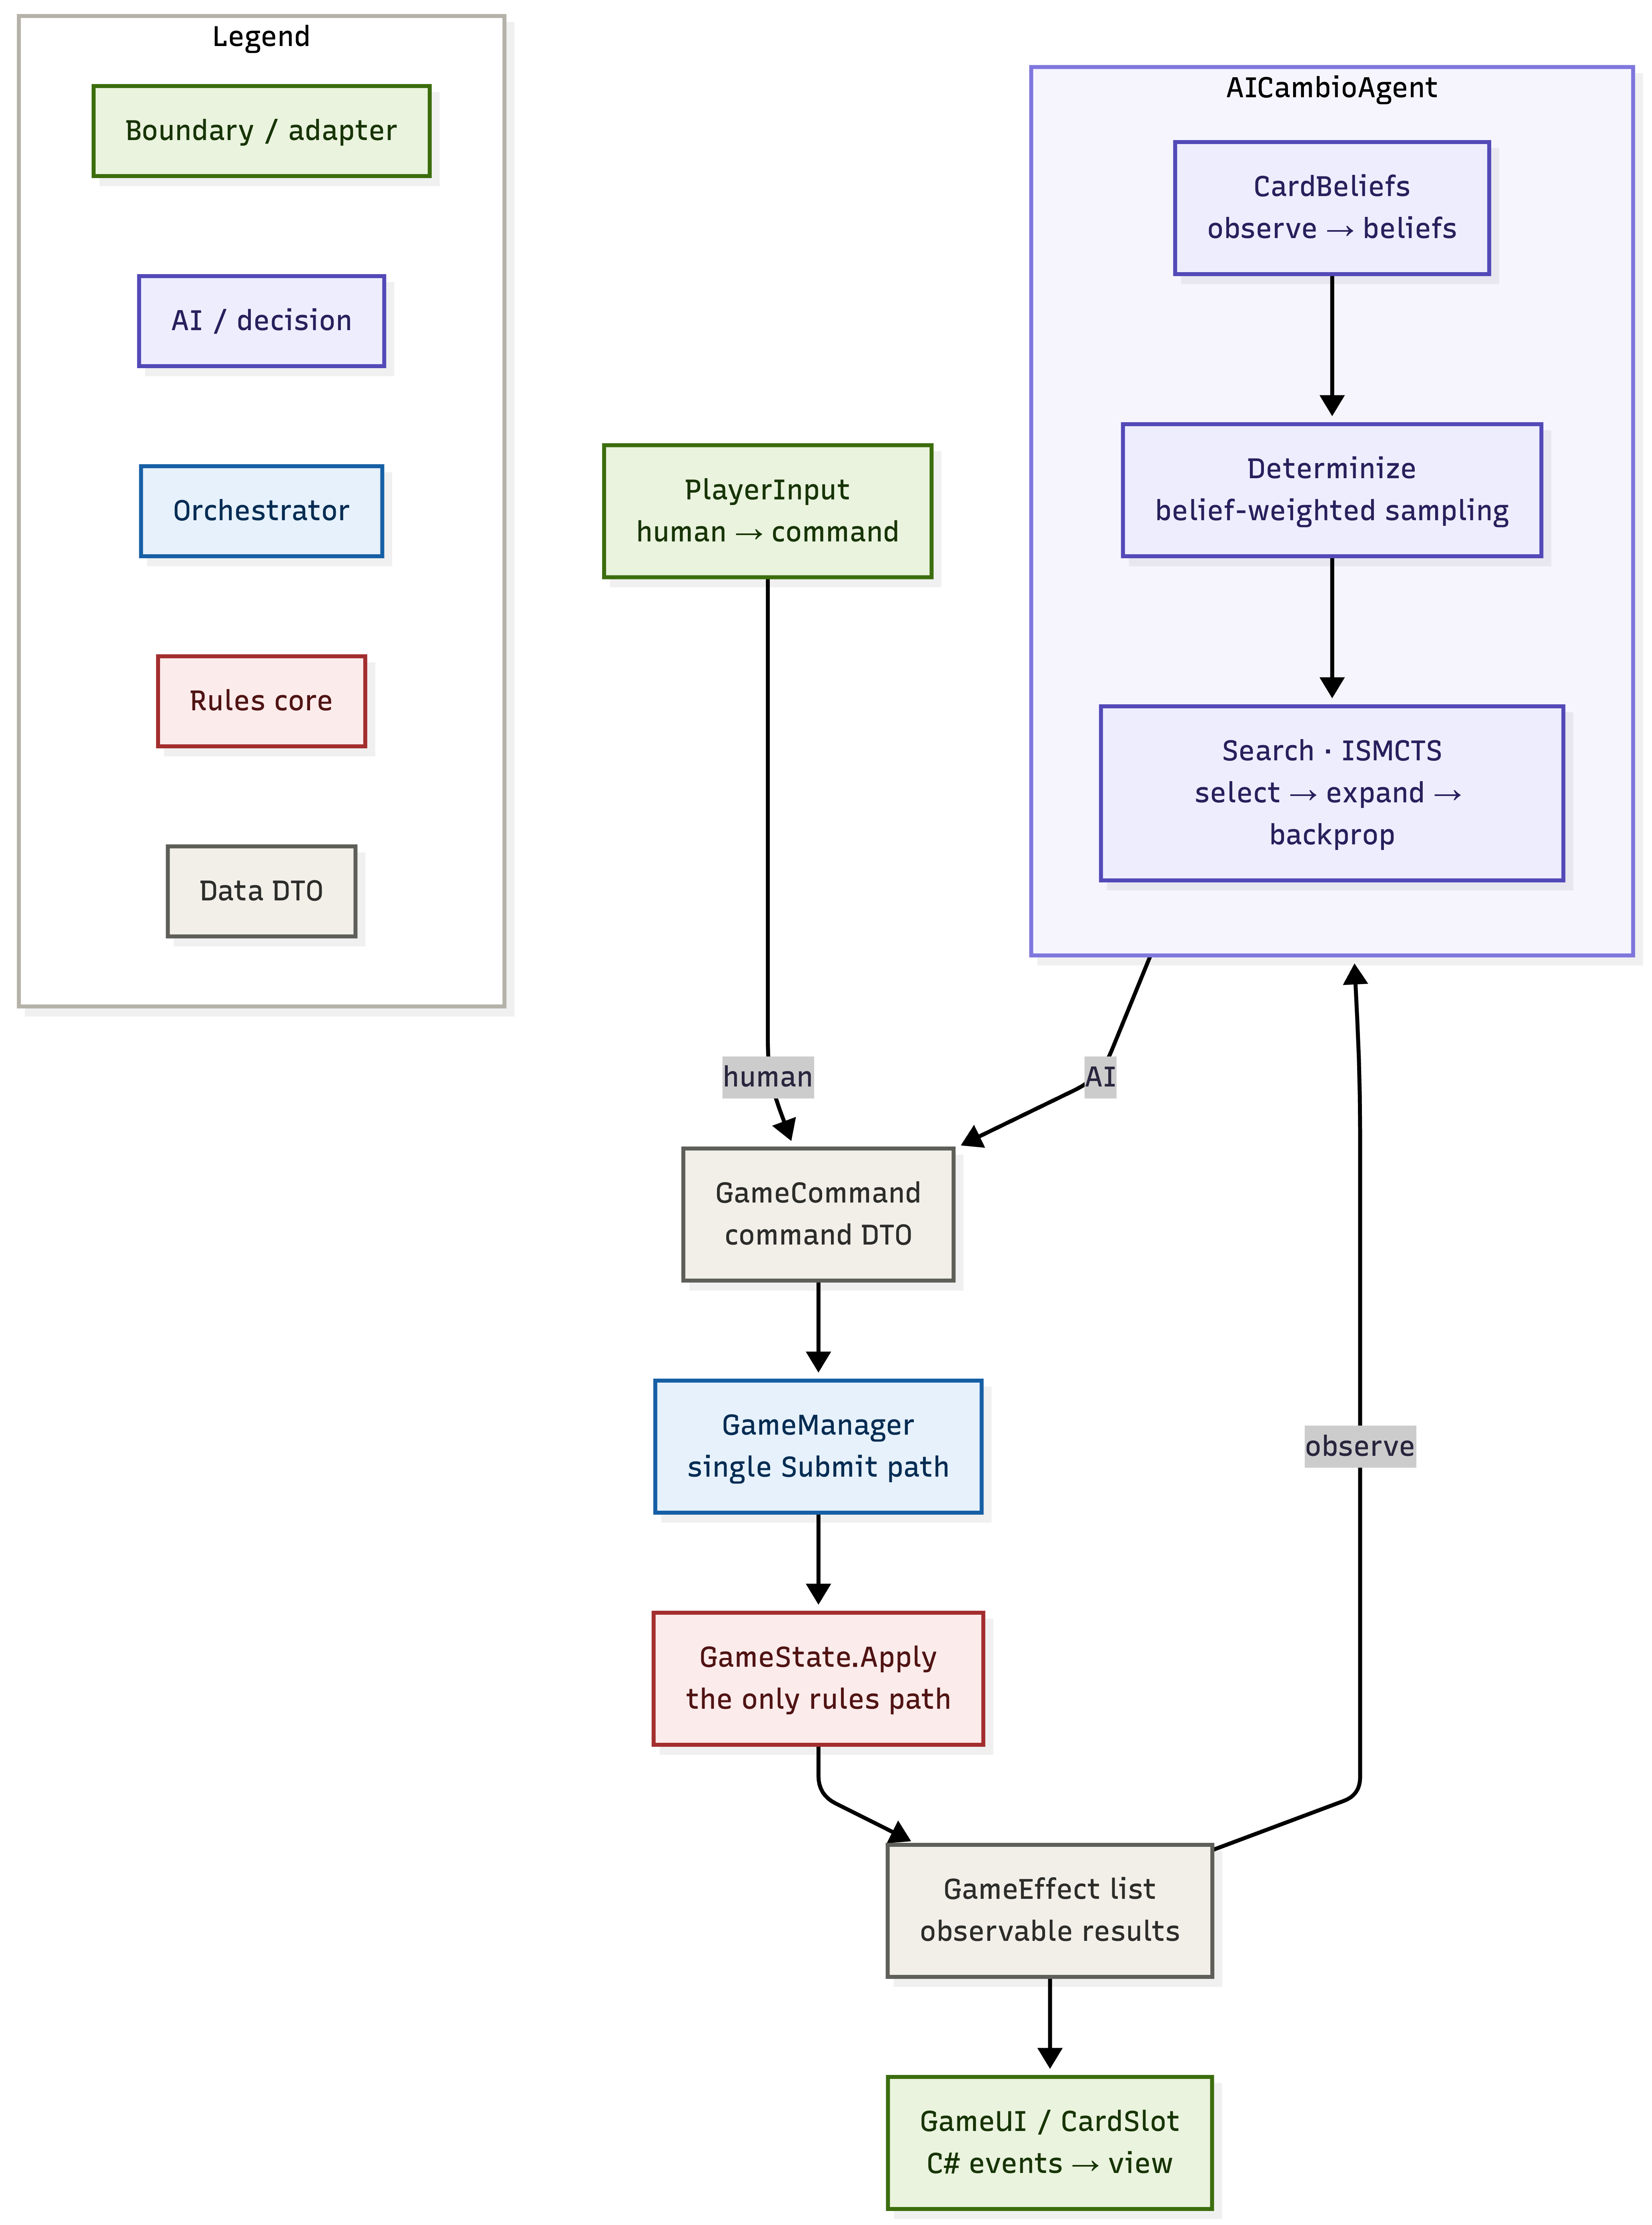
\includegraphics[width=\textwidth]{images/general_flow_chart.png}
    \caption{Overview of the system architecture, tracing a single action from either participant through the game engine to its observable effects.}
    \label{fig:architecture}
\end{figure}

Figure~\ref{fig:architecture} provides an overview of the system architecture, focusing on how a single action flows from either participant through the game and produces observable results. The human player and AI agent are treated as interchangeable drivers of the same game engine. Each expresses its chosen action as a command, which is submitted through a single path and applied by the only code permitted to modify the game state. The resulting changes are then reported as a stream of observable effects that drive both the game view and the agent's beliefs. Chapter~\ref{chap:design} describes the implementation of this path and explains how it ensures live gameplay and the search operate under the same rules.

\section{Evaluation Methodology}
\label{sec:eval-method}

\subsection{User Study Design}
This project aims to recruit 20 participants to play-test both AIs. Each tester plays
20 games in total, yielding approximately 400 data samples,
enough to draw an objective conclusion about the project.

The testing procedure gives each player complete freedom in choosing their first
opponent. Because the players are never told which AI is the baseline ISMCTS and
which is the Bayesian variant, this choice is effectively random. Preserving this
blindness matters: it removes bias when players later report which AI they
preferred, since revealing which one contains my contribution could make them more
generous when rating it.

To measure how players perceive the AIs, a Google Forms questionnaire was designed to gather qualitative information about their gameplay experiences, which is then related to the objective behavioural metrics to reach a well-founded conclusion. The questionnaire first collects background information about each participant, including their familiarity with video games and card games, to assess how this may affect their perception of the AI. The same questions are asked about both AIs to ensure a fair comparison, followed by a question asking which AI the participant preferred or whether they remained neutral. The proposed questions are as follows:

\paragraph{Background.}
\begin{enumerate}
  \item Do you play video games?
  \item Do you play card/board games?
  \item Have you played card games similar to Golf, Skyjo or Poker?
  \item Have you played Cambio before?
  \item Please select your age group.
\end{enumerate}
Questions 1 and 2 offer four options ranging from ``Yes, regularly'' to ``No'';
questions 3 and 4 are yes/no; and question 5 offers age groups from 18 to 50+.

\paragraph{AI evaluation (asked identically for each AI).}
\begin{enumerate}
  \item Did you enjoy playing against (AI Name)?
  \item Do you feel (AI Name) adjusted its strategy based on how you were playing?
  \item Did (AI Name) feel predictable at any moment during the match?
  \item Did (AI Name) feel like it had a strategy?
  \item Did (AI Name) respond differently when you used special cards such as peek
        or swap?
  \item Do you feel (AI Name) took too long to play?
\end{enumerate}
Question 5 has the options yes, no and neutral; the remaining questions use a
four-point Likert scale of strongly disagree, disagree, agree and strongly agree.

\paragraph{Preference.}
\begin{enumerate}
  \item Which AI did you feel was more interesting and fun to play against?
\end{enumerate}
The options are either AI or neutral.

The responses are analysed using a Wilcoxon signed-rank test because the data are paired, with each participant rating both AIs, and ordinal, as they are collected using a Likert scale. The data are also not assumed to be normally distributed, making a non-parametric paired test appropriate. The same rationale is applied to the paired tests used through out the evaluation. The complete questionnaire is provided in the appendix.

\subsection{Behavioural Metrics}
\label{sec:behav-metrics}

The behavioural metrics capture how the AIs approach the game. They provide the objective side of the evaluation, with an in-game telemetry layer recording every relevant AI action in a set of CSV files. This makes it possible to assess which agent performs better independently of player perceptions and then compare the behavioural results with the questionnaire responses.

Only the AI’s own actions are logged. The human opponent is treated as a confounding factor rather than a subject of analysis, preventing differences between individual human players from affecting the comparison between the two agents. The telemetry is stored across three CSV tables, all of which can be joined using `(session\_id, match\_index)`.


The telemetry is organised into three tables. The \texttt{cambio\_matches} table holds one row per game: the outcome (winner and both scores) together with the AI's behaviour that match, including how often it swaps versus discards, the average value change of its swaps, its matching accuracy and penalties, its use of power cards, its mean number of still-hidden own cards, and its mean decision time. The \texttt{cambio\_calls} table holds one row per game in which Cambio was called, recording who called, on which turn, the scores at that instant, whether the caller was actually ahead, and the believed-score variable each guard used to justify the call. The \texttt{cambio\_beliefs} table holds one row per hidden card per decision and is the data produced by the Bayesian layer: for each uncertain card it logs the belief-driven shift the layer applies to that card's expected value (the \emph{tilt}) against the card's ground-truth value, so that the calibration of the layer can be measured. Because the tilt is identically zero when the Bayesian layer is disabled, these rows act as a null control that isolates exactly what the layer adds. All three tables share the session and match keys that let them be joined, and the complete column dictionary is given in Appendix~\ref{app:telemetry}.

\paragraph{Cambio-call table (\texttt{cambio\_calls})}
This justifies each agent's decision to end the game on its own terms. It records
who called and on which turn (\texttt{cambio\_caller},
\texttt{cambio\_caller\_turn}), the scores at that instant, and whether the caller
was actually ahead (\texttt{cambio\_caller\_was\_ahead}), that is, whether the call
was correct. It also stores the variable each guard used to justify the call: the
baseline's flat believed-own-score (\texttt{cambio\_ai\_believed\_score}), and, for
the Bayesian agent, the believed own and opponent end-score means together with the
probability of finishing ahead (\texttt{guard\_believed\_own\_mean},
\texttt{guard\_believed\_opp\_mean}, \texttt{guard\_p\_ahead}).

\paragraph{Belief table (\texttt{cambio\_beliefs}), one row per hidden card per AI
decision.}
This is the additional data produced by the Bayesian layer, and it validates the
per-card value estimates that the layer feeds into the search. For every card the
AI is uncertain about, it logs whether the card belongs to the opponent
(\texttt{is\_opponent\_slot}), whether the opponent is believed to know it
(\texttt{opp\_knows}), the card's ground-truth value (\texttt{true\_value}), and two
\emph{tilt} values: \texttt{tilt\_raw}, the shift the belief layer applies to that
card's expected value relative to a flat deck prior, and \texttt{tilt\_eff}, the
shift the search actually consumed. Comparing the tilt against \texttt{true\_value}
measures the calibration of the layer: a card believed to be low should, on
average, actually be low. Crucially, when the Bayesian layer is disabled the tilt
is identically zero, so these rows act as a null control and let me quantify exactly
what the layer adds.

\paragraph{Statistical testing.}
The behavioural data are compared with a Mann-Whitney U test. Although each participant faces both agents, the two agents were evaluated over independent sets of games of unequal size, so the observations cannot be paired at the game level. The belief-calibration metrics (the raw and effective tilt against ground truth) are tested the same way, with the zero-tilt rows produced when the Bayesian layer is disabled acting as the null control described above.

\subsection{Computational Metrics}
\label{sec:comp-metrics}
Whether the AI is computationally optimal reduces, for the purposes of this project,
to its play time and the speed of the tree search. The design target is a very low
hardware requirement so that the game runs on as many laptops as possible, and the
telemetry captures this directly through \texttt{ai\_decision\_ms\_avg}, the mean
wall-clock time the search spends per decision. The search reporter additionally
exposes the number of iterations completed against the target and the number of
nodes expanded, which help explain that timing.

Because the Bayesian layer adds the belief update and the distribution-based Cambio
guard on top of the search, comparing \texttt{ai\_decision\_ms\_avg} between the two
agents also quantifies the runtime overhead that my contribution introduces; the
same paired Wilcoxon test applies here.

Frames per second and other real-time benchmark metrics are irrelevant to this
study, because the game is turn-based, with the small exception of the brief
real-time window in which the AI may attempt a match during the opponent's turn.

%============================================================================
%  CHAPTER 4 -- DESIGN AND IMPLEMENTATION  (restructured to match the codebase)
%============================================================================
\chapter{Design and Implementation}\label{chap:design}
\label{ch:impl}

This chapter describes how the system was designed and built. To explain it better, I organised it into three layers that mirror the experimental design of the study. The first layer, covered in Sections~\ref{sec:mutation-path}--\ref{sec:determinization}, is the shared foundation used by both agents: the game core and its single mutation path, the card model and scoring, and the determinization support that lets a hidden state be sampled and searched. 

The second layer, in Section~\ref{sec:ismcts}, is the baseline ISMCTS agent, which works as a baseline for the Bayesian layer and can also operate independently. The third layer, in Sections~\ref{sec:beliefs}--\ref{sec:cambio-guard}, is the contribution of this dissertation, which is split as follows: the belief layer, the belief-weighted determinization that feeds those beliefs into the search, and the distribution-based Cambio guard. The chapter then covers how the agent is integrated into Unity, how the variety and unpredictability the study probes actually arise, and how the system is instrumented.

The important point to keep in mind throughout is that the control and the contribution are not two separate agents but the same engine with the belief machinery switched off or on. In the code, this is controlled by a single toggle. When false, the agent samples hidden states uniformly and calls Cambio on a flat absolute cap; when true, the same agent samples according to its beliefs and calls Cambio using a relative, distribution-based test (Bayesian layer). Presenting the baseline first and then layering the Bayesian components on top reflects exactly this relationship, and it is what makes any measured difference between the two attributable to the belief machinery alone.


\section{Architecture Overview and the Single Mutation Path}
\label{sec:mutation-path}

This section explains how the formalisation of Cambio is implemented in code, in particular how actions are dispatched, what is permitted to modify the state, and how the results of those modifications reach the two different consumers, players and AI. The entire design architecture is built so there is only one way to modify the game state. Figure~\ref{fig:architecture} traces the path of a single action, and the remainder of this section follows that path in order.

The state itself is contained within \texttt{GameState}, which stores the layout as plain data, including the hand and penalty slots for both sides, the draw and discard piles, whose turn it is, the current \texttt{GamePhase}, the card currently drawn, the power being resolved, and the endgame flags associated with a called Cambio. All are private to prevent both the player and the AI from directly accessing the value of a hidden card; the data the outside world may need is exposed as public read-only.

Both the player and the AI interact with this same state through the same action vocabulary. Every possible action is represented as a \texttt{GameCommand}, which combines a \texttt{CommandType} (drawing, discarding, swapping the drawn card, using a power, attempting a match, giving a card, confirming a trade, finishing a peek, or calling Cambio) with an optional \texttt{SlotRef}. The slot reference identifies a target using its side, zone, and index, forming a numeric value in the form of  “(X, X, X)”. The player and the AI produce these commands in different ways but ultimately use the same interface: the player through game clicks and the AI through the ISMCTS search. This makes them interchangeable drivers of the same game engine and ensures that both agents being compared, as well as the human opponent, are restricted to the same set of legal actions.\texttt{GameState.LegalMoves} examines the current phase and returns the valid commands, and this same set forms the branching factor enumerated by the search at each node.

Every command, regardless of its source, is submitted through \texttt{GameManager}, which is the only object that interacts with the live state, and is applied using the method  \texttt{GameState.Apply}. This provides the single mutation path through the implementation and represents the most important structural decision in the system. 

\texttt{Apply} dispatches each command to the appropriate internal handler, which first validates the command against the current phase before modifying the state. For example, a discard is rejected if no card has been drawn, while a Cambio call is rejected unless the game is in the drawing phase and a call has not already been made. If validation fails, the state remains unchanged. If validation succeeds, the handler applies the required changes and records what occurred. 

This structure is important to highlight because the same implementation serves two different purposes. During live play, \texttt{Apply} advances the real game, while during search the AI clones the state and uses the same \texttt{Apply} method to advance simulated games. Because there is only one implementation of the game rules, a simulated Cambio behaves in the same way as a real game, with no separate simulation logic that could diverge from the live implementation as the code develops. This is key because the belief and opponent-modelling layers introduced later in this chapter rely on simulated outcomes, which are only meaningful when the simulation accurately represents the game being played.

Applying a command modifies the state and returns a list of \texttt{GameEffect} values that describe the observable consequences of the action. Each effect is a small record representing something that could have been observed during play, such as a card being drawn, a slot being revealed to a particular side, two slots being swapped, a match being resolved, etc. This effect stream provides the system's single representation of observable events and is consumed by two separate audiences. The first is the game view. \texttt{GameManager} dispatches each effect as a C\# event, which the Unity UI subscribes to and uses to update the presentation. The second audience is the agent. Its \texttt{CardBeliefs} component receives the same effects through its \texttt{Observe} method and preventing the belief layer from accessing information that the agent should not know. \texttt{CardBeliefs} never reads \texttt{GameState} directly and instead learns about the game exclusively through the effect stream, which represents the information available to an observer of the game. It only updates its belief about a revealed card when the relevant side was entitled to observe its value.

This completes the loop on which the remainder of the chapter is built. The agent produces a command, submits it through the same mechanism used by the human player, observes the effects, and updates its beliefs before selecting its next action. The uniform baseline and Bayesian variant differ only in how those beliefs are used when sampling hidden states.



\section{Card Model and Scoring}
\label{sec:card-model}

A card is the smallest unit of state in the game; rather than storing rank, colour, value, and power as separate fields, a \texttt{Card} is represented by a single integer identifier, with all other properties derived from it arithmetically when required. This keeps cards inexpensive to copy across the thousands of determinizations the search clones, and lets the determinizer sample a single value per hidden slot rather than juggling several fields that could become inconsistent. The trade-off is that the decoding logic depends on the identifier layout remaining fixed: any change to how ranks, colours, jokers, and the empty-slot sentinel are packed into the identifier would require the derivation formulas to be updated accordingly.


\section{Determinization Support}
\label{sec:determinization}

The way determinization allows an imperfect information game to be tackled as a perfect information one is that, before each simulation, the unknown parts of the state are assigned concrete values to produce a fully specified world that can then be searched as though all information were visible. This section describes the supporting functionality in \texttt{GameState} that produces such a world, while leaving aside the question of how the hidden values are selected. This separation is important because the uniform baseline and the belief-weighted sampler differ only in their sampling policies, while the surrounding determinization machinery remains identical.

The process begins with \texttt{Clone}, which creates a deep copy of the public state using a fresh seed derived from the iteration number, which ensures that successive determinizations can produce different worlds. All simulation then takes place on the cloned state, without altering the outside world. 

\texttt{UnseenCardIds} provides the pool of cards available to fill the hidden slots. It contains every identifier that is not currently known, is not in the discard pile, and is not the card currently being held as the drawn card. The hidden slots are then assigned concrete cards through \texttt{OverwriteHidden}, while the remaining cards are placed into the future draw order through \texttt{SetDrawPile}. This preserves the distinction established in Chapter~\ref{chap:methodology}, where the sampling policy is applied to hidden slots while the draw pile is treated as carrying no evidence.

The method \texttt{IsCardSetWorking} provides a consistency check by verifying that every identifier appears exactly once across all slots, both piles, and the currently drawn card. If the resulting world fails this validation, the agent can discard it rather than allowing an impossible state to enter the search, reducing the amount of noise in the search.

\section{The Baseline ISMCTS Agent}
\label{sec:ismcts}

The baseline agent is a standard ISMCTS implementation, and it is described here only to the extent required to understand the contribution that follows. Implementing ISMCTS is not itself a goal of this project. Instead, it provides the control condition against which the belief machinery in Sections~\ref{sec:beliefs} and~\ref{sec:bayesian} is evaluated. The purpose of this section is therefore to establish how the agent makes decisions when it has no beliefs about hidden information. 

A single decision is produced by running many search iterations over a shared tree, with four thousand iterations used by default, before selecting the most-visited move at the root. This figure was chosen empirically during development. Once the Cambio Guard of Section~\ref{sec:cambio-guard} is applied, four thousand iterations proved sufficient for the agent to simulate enough games to reach a competent decision, while remaining low enough to keep a single decision within roughly 500 to 1500 milliseconds. This is comfortably fast for a turn in a card game, where the agent is not competing for a real-time frame budget. Keeping the iteration count low also allowed the game to be developed and tested quickly without waiting for the search.
 Each iteration begins by using the determinization functionality described in Section~\ref{sec:determinization} to sample a concrete world consistent with the information available to the agent. The search descends through the tree using the selection policy until it reaches a node with an untried move, expands a new node, evaluates the resulting position, and propagates the evaluation back through the visited path. Since a different world can be sampled on each iteration, the shared tree accumulates statistics across multiple possible states rather than representing a single fixed board. This allows the tree to represent an information set rather than a single fully known state. 

Selection uses Upper Confidence Bound applied to Trees, balancing exploitation of moves that have performed well with exploration of moves that have been visited less frequently. Rewards are stored from the AI's perspective throughout the tree. When the selected node belongs to the opponent, the exploitation term is inverted so that the opponent is modelled as attempting to minimise the AI's reward rather than maximise it. This maintains the adversarial nature of the search without requiring separate reward statistics for each player.

Evaluation reflects what the agent prefers. Terminal positions receive a simple win, draw, or loss score. A non-terminal leaf, which is the more common case given the relatively short search horizon, is evaluated by combining two terms: how far ahead the agent is compared with the opponent, with the result passed through a $\tanh$ function so that a small advantage is rewarded while larger advantages gradually saturate and how low the agent's own hand is relative to a target score, again using a saturating function plus a penalty for any “penalty cards” held by the agent. The reason to measure how low the agent's hand is as an absolute number is to provide an additional incentive to continue reducing its own hand and not get satisfied with an average hand. Together, these terms favour positions in which the agent is both ahead of the opponent and objectively in a strong position.

With the Bayesian layer disabled, each unknown slot is filled by drawing uniformly from the unseen pool, treating every card consistent with the available information as equally likely. This is the standard ISMCTS determinization approach and the control condition against which the belief-weighted variant is measured.

\section{The Belief Layer}
\label{sec:beliefs}

Standard ISMCTS reasons about hidden information without ever committing to what that
information is likely to be. Each search iteration guesses a complete state and searches
it, with the guesses being drawn without any preference or likelihood. The belief layer
is the first half of this dissertation's contribution. Its purpose is to give the agent
an explicit, continuously updated view of the cards it cannot see, so that these guesses
can later be made in an informed way rather than blindly.

The layer maintains one of two states for every card in play. A slot is either known,
meaning the agent has legitimately seen the card and therefore knows its value with
certainty, or hidden, in which case the agent maintains a probabilistic belief about
which value the slot is likely to contain. These beliefs are based only on information
the agent is actually entitled to use, including cards it has seen through its own looks
and powers, as well as inferences drawn from the opponent's visible choices. The agent
never accesses the true value of a hidden slot, so the belief layer models the game from
the same limited perspective available to a human player. The remainder of this section
explains how these beliefs are represented, how they are updated in response to
observable events, and how the opponent's behaviour is incorporated as evidence. How
these beliefs are subsequently used by the search is discussed in
Section~\ref{sec:bayesian}.

\subsection{Representation}

For each hidden slot, the layer maintains an accumulated log-likelihood vector over the twelve possible card values; card values range from -1 to 10, and these values are mapped to buckets using the index v+1. Each entry represents the extent to which the evidence gathered so far supports or contradicts the possibility that the slot contains a card of that value. The evidence is stored additively in log-space, allowing independent observations to be combined through addition rather than requiring probabilities to be multiplied directly.

For this representation to work, we need a neutral state which would be a vector containing only zeros, meaning it expresses no preference among the possible values and represents a slot for which no evidence has been gathered. When the layer is queried for a slot's log-likelihood, it returns this flat vector unless evidence has changed it. An uninformed slot therefore contributes no additional preference of its own and instead relies entirely on the deck prior when the determinizer combines the two (Equation~\ref{eq:posterior}). The same handling applies to known slots.

\subsection{Updating Beliefs from Observed Effects}

Beliefs are updated by the effect stream. Each \texttt{GameEffect} produced by the game is passed to the belief layer together with a flag indicating whether the agent was the actor responsible for the action or not. The layer then updates itself using this information. This flag is important because it allows the layer to distinguish between information the agent is entitled to know and information that it may have observed without being allowed to see the underlying card, preventing cheating.

Let's analyse when a card is revealed to see the flow of information. When a slot is revealed, the layer records the card as known when the agent was the side that acted. A reveal triggered by the opponent therefore does not give the agent knowledge of the card's value, even though the agent can observe that the reveal occurred. Swaps also move knowledge together with the card. When two slots exchange their contents, any known information or belief associated with the cards moves to their new locations, allowing a card that has already been identified to remain known after being moved. When the drawn card is swapped into a slot, the handling depends on which side acted; in the case the agent performs the swap, it records the card that it placed; otherwise, the inserted card remains hidden, and the action instead provides behavioural evidence, as described below.

Matches are handled similarly. When a match succeeds and a card leaves a slot, the corresponding slot is cleared. When a match fails, the mismatched card is revealed to both sides and is therefore recorded as known. Across all of these cases, the same principle is maintained. Certainty is granted only when the agent has accessed the card's value, while any evidence associated with a slot is discarded whenever the contents of that slot change. 

\subsection{The Opponent-Evidence Model}

The true depth of this opponent model is that it also reads meaning into the opponent's choices, treating
each observable decision as evidence that shifts the belief about otherwise unseen cards.
This is the mechanism by which the agent adapts to the particular player in front of it
rather than assuming, introducing concepts of Dynamic Difficulty Adjustment (DDA). Three signals are modelled, each expressed as an additive shift to the
relevant log-likelihood vectors, and each deliberately bounded so that no single observation can overwhelm the rest of the evidence.

The strongest is the keep signal. When the opponent draws a card and
chooses to keep it, that choice is informative, and the model guesses that a
rational player only keeps a drawn card if it improves on what they gave up. The displaced
card's value is public, so the player leans the hidden slot's belief towards values below
it, sharply for values well under the discarded one and gently for values close to it,
using a sigmoid on the gap between the two, plus a small blanket lean-low reflecting that
the mere act of keeping a draw is itself weak evidence the card is good for them. 

The second signal comes from persistence. A slot the opponent is believed to know and has left
untouched across several turns is probably one they want to keep, so the layer applies
a gentle lean-low that grows with the number of turns the card has stayed untouched, up to a cap so
that a long game does not let this accumulate without limit. The third signal analyses when the opponent discards a low card face-up; this is weak evidence that their hand as a whole is running low, so a small lean-low is applied across all of their slots at once, scaled by how far below a typical value the discard was and again held under a ceiling.

Each of these is only ever a lean, never a certainty. They bias which worlds the search
spends its effort on without ever ruling a physically possible card out, and because they
are read from the specific opponent's specific choices, two different players who play the
same position differently will push the agent's beliefs in different directions. This is
the concrete sense in which the agent answers to how a human is  playing,
which is the behaviour the research question sets out to test.


\section{Belief-Weighted Determinization}
\label{sec:bayesian}
 
This section presents the core of the contribution, the mechanism that connects the beliefs described in Section~\ref{sec:beliefs} to the ISMCTS search described in Section~\ref{sec:ismcts}, moving from treating every possible hidden configuration as equally plausible to focusing its search on the worlds it has reason to believe are most likely to be true. The complete pipeline is shown in Figure~\ref{fig:determinization}.

\begin{figure}[H]
    \centering
    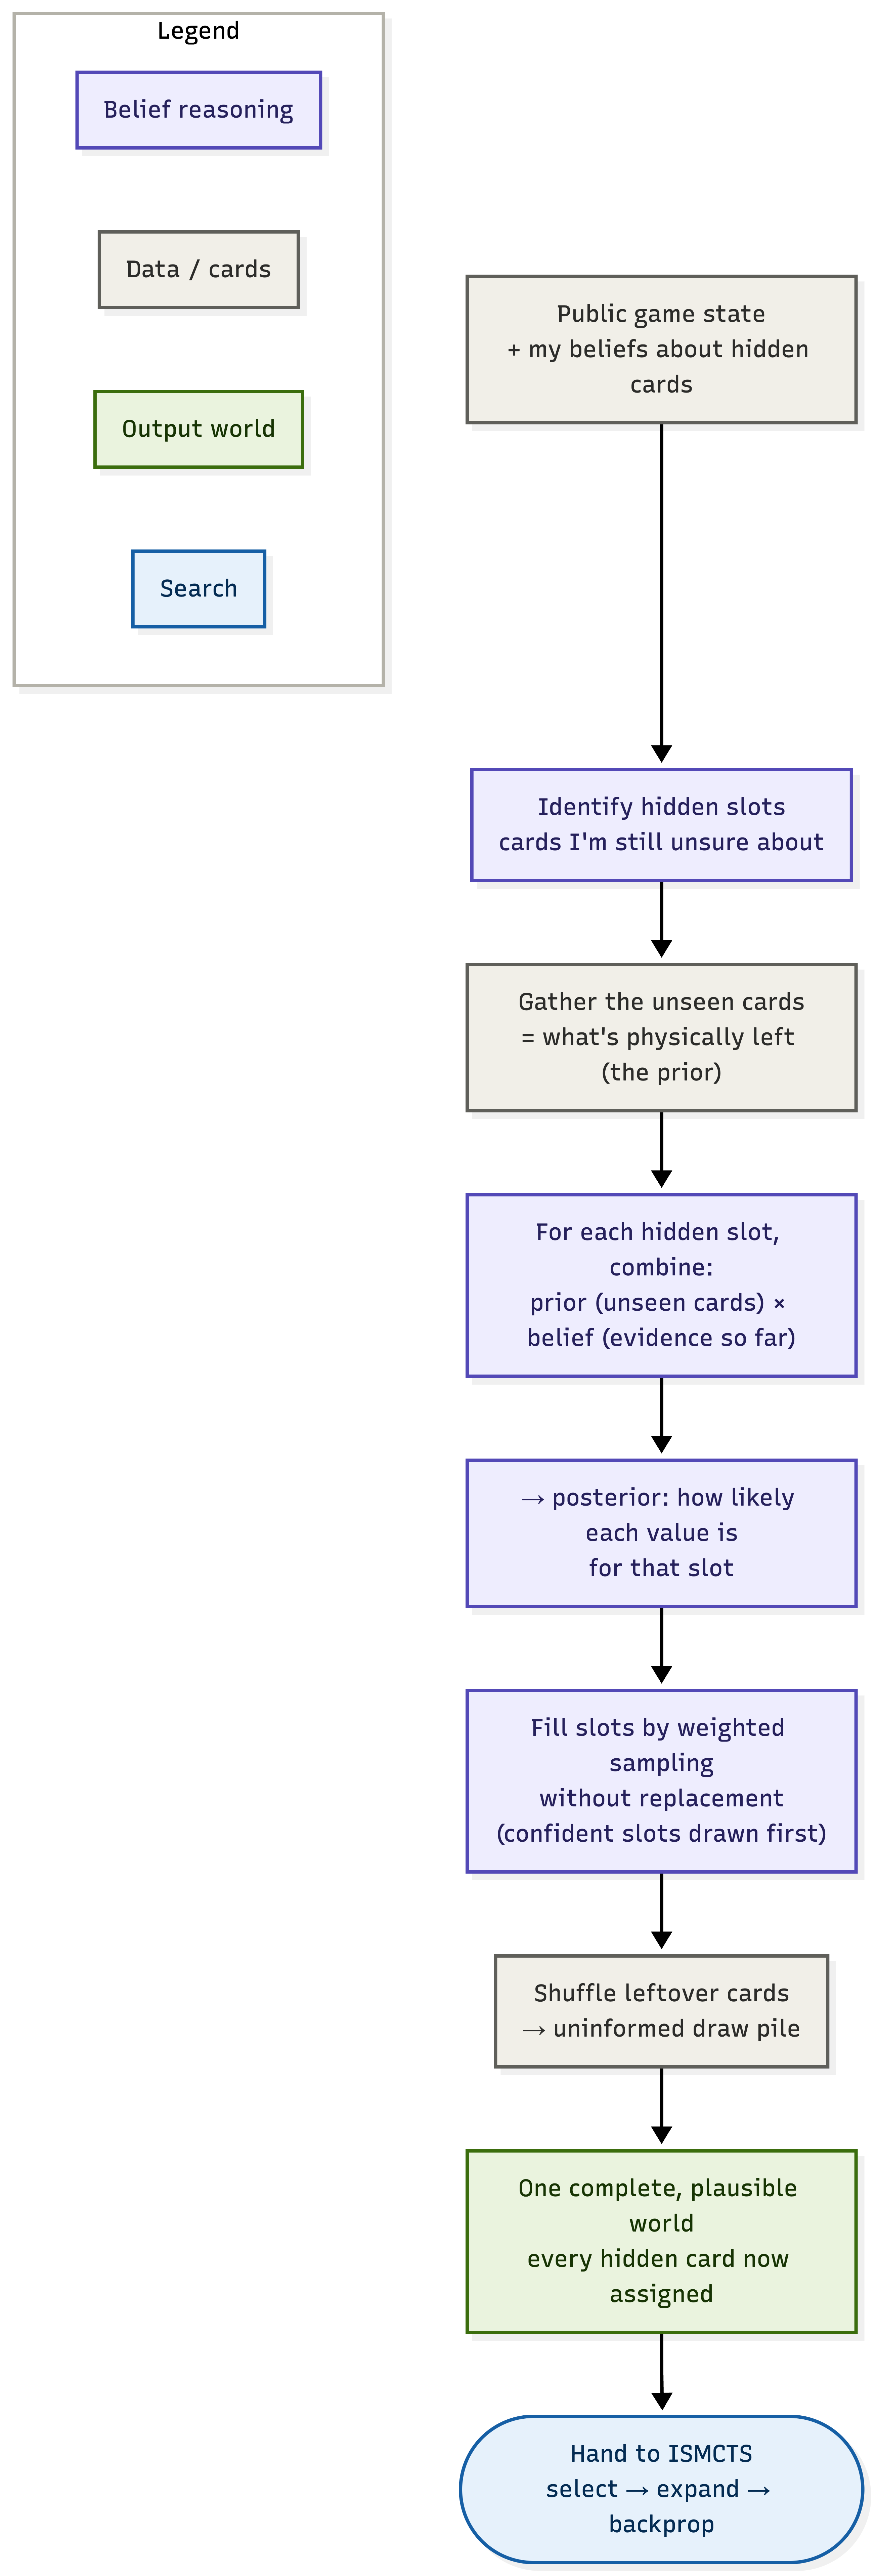
\includegraphics[width=0.5\textwidth]{images/determinization_flow.png}
    \caption{The belief-weighted determinization pipeline.}
    \label{fig:determinization}
\end{figure}
 

\subsection{The Posterior Where Prior Meets Evidence}
 
The foundational idea behind the design is that the physical set of cards not yet accounted for constitutes the unseen pool. If the agent knows the location of certain cards, then every remaining card must be distributed among the hidden slots and the draw pile, and the composition of that pool dictates how likely each value is before any behavioural evidence is considered. A value that appears many times in the remaining pool is, all else being equal, more likely to occupy a given hidden slot than a value that appears once.
 
Combining that pool with the per-slot log-likelihood vector from Section~\ref{sec:beliefs} gives a per-slot posterior over values,
%
\begin{equation}
  P(\text{slot} = v) \;\propto\; N_{\text{pool}}(v)\,\exp\!\big(\ell(v)\big),
  \label{eq:posterior}
\end{equation}
%
Here, $N_{\text{pool}}(v)$ represents the number of cards of value $v$ that remain in the unseen pool, while $\ell(v)$ represents the accumulated log-likelihood for that value in the slot. When the log-likelihood is flat, as it always is when the Bayesian layer is disabled or when no evidence has been gathered about a slot, the exponential term is constant. The posterior therefore reduces to the pool prior alone, which is exactly the behaviour of the uniform determinizer. This makes it so when it uses a flat belief the two agents sample identically. The belief layer adds evidence on top of the deck's natural distribution without contradicting it. A card that is physically impossible because it is absent from the pool can never be sampled, regardless of how strongly the belief favours it, since its prior count is zero.

 
\subsection{Sampling One World}
 
A single determinization follows the pipeline shown in Figure~\ref{fig:determinization}. The agent first clones the public state using a fresh random seed derived from the iteration number, ensuring that successive iterations explore different worlds. It then identifies the hidden slots, including every active slot on either side, and constructs the unseen pool from the concrete list of card identities that have not been assigned to a known location to later apply a consistency check. If the pool contains fewer cards than the number of hidden slots, or if the resulting card multiset fails validation, the world is discarded, and the iteration is skipped rather than allowing an impossible state to corrupt the search.
 
The hidden slots are then filled one at a time using weighted sampling without replacement. For each slot, the effective log-likelihood is calculated by combining the stored belief for that slot with a situational adjustment described below. This value is then exponentiated to produce a weight for each possible card value. Each remaining card in the pool is assigned a weight based on the value it carries, and one card is sampled in proportion to these weights before being removed from the pool, preventing the same card from being assigned to multiple slots. Sampling without replacement is essential since the same physical card cannot occupy two locations. Removing each card as it is placed ensures that every sampled world remains internally consistent with a real deck.
 
In order to make this process more robust, I added two details. First, the exponentiation uses a max-subtraction, computing $\exp(\ell(v) - \max_u \ell(u))$ rather than $\exp(\ell(v))$ directly. The common offset cancels out in the sampling ratio, while the shift prevents numerical overflow when a belief is strongly concentrated on a particular value. Second, the hidden slots are not filled in an arbitrary order. Because sampling without replacement is order-sensitive, cards assigned to earlier slots are unavailable to later ones. The agent therefore sorts the hidden slots according to the strength of their beliefs and fills the most confident slots first. A slot whose posterior is strongly concentrated on a particular value has the most to lose if that value is assigned to a slot with no strong preference. Filling the most confident slots first therefore reduces the bias introduced by naive sequential sampling. Slots with no evidence and a flat belief are filled last, taking whatever cards remain. This is the appropriate behaviour because these slots express no preference between the available values.

 
Once every hidden slot has been assigned, the remaining cards in the pool become the draw pile. The order of the draw pile contains no evidence, since nothing the agent has observed constrains which unseen card will be drawn next. The remaining pool is then shuffled uniformly and used as an uninformed draw order. This produces a plausible world in which each hidden card has been assigned according to the posterior, while the future draw order remains random. This world is passed to ISMCTS for a single selection, expansion, and backpropagation pass. Across the thousands of iterations used to make a decision, the search therefore encounters a distribution of worlds that reflects the agent’s beliefs and concentrates its effort on the configurations that the available evidence suggests are most likely.
 
 
%----------------------------------------------------------------------------
\section{The Cambio Guard}
\label{sec:cambio-guard}

During development, standard ISMCTS treated calling Cambio in the very first or
second round as a reasonable strategy, and so it did so very often. While an
early call can occasionally be effective, the repetition made it clear that this
was not a healthy or realistic way to approach the game. At that stage, the
decision is essentially a blind RNG gamble, resting entirely on the total number
of cards in the deck and the possible combinations rather than on any acquired
knowledge of the hand.

To prevent this, I developed the Cambio Guard. In essence, it is a filter applied
to the root move set of the search. While the AI does not yet believe its own
hand is low enough, the \texttt{CallCambio} move is removed from the legal actions
the search is allowed to consider, forcing the AI to keep playing until its
believed hand value reaches the threshold or falls below it. In its baseline form,
the guard is an absolute cap; the summed believed own score must be less than or
equal to \texttt{CambioGuardScore}, whose default value is $10$, since that gave
the best Cambio-calling behaviour:
%
\begin{equation}
  \sum_{s \in \text{own slots}} \widehat{\text{value}}(s) \;\le\; \texttt{CambioGuardScore}.
\end{equation}
%
This believed score uses a flat prior: slots the AI is certain of contribute their
exact value, and every unknown own slot contributes a fixed prior value, which is
$5.889$:
%
\begin{equation}
  \widehat{\text{value}}(s) =
  \begin{cases}
    \text{value}(s) & \text{if $s$ is known,}\\[4pt]
    5.889           & \text{if $s$ is unknown.}
  \end{cases}
\end{equation}
%
Another key feature to stand out is that Cambio Guard will never filter the move
set down to zero; if removing the call would leave no legal moves, the call is
left in.

This does interfere with the way ISMCTS ordinarily reaches decisions via selection
policy (UCT). By pruning \texttt{CallCambio} at the root, the guard overrides that
reward-driven choice in this one narrow case. In the context of Cambio, this
produced a markedly better experience since the game involves very few variables:
each player holds only four cards and starts the game with just two unknowns. In
such a small state space, a hard behavioural prior is a reasonable substitute for
what the search cannot reliably learn from so little information.

This became a key aspect of my design, because the moment of calling Cambio also
became dynamic and belief-based within my Bayesian layer. Standard ISMCTS decides
whether to call Cambio purely on how good its hand is in absolute terms, with no
regard for how weak the opponent's hand might be. The Bayesian variant instead
replaces the absolute cap with a relative, distribution-based test. It estimates
believed end-score distributions for both itself and the opponent under the same
deck coherent posterior, where known slots contribute their exact value with zero
variance, and each hidden slot contributes a mean and variance drawn from the
posterior
%
\begin{equation}
  P(v) \;\propto\; \texttt{poolHist}[v]\cdot\exp\!\big(\texttt{effLogL}[v]\big),
\end{equation}
%
combining what remains in the unseen pool with the accumulated likelihood
evidence. The difference between the two hands,
%
\begin{equation}
  D = \text{own} - \text{opponent},
\end{equation}
%
is modelled as a Normal distribution whose mean is $\mathbb{E}[\text{own}] -
\mathbb{E}[\text{opp}]$ and whose variance is $\operatorname{Var}[\text{own}] +
\operatorname{Var}[\text{opp}]$ (a mean-field approximation treating the two hands
as independent):
%
\begin{equation}
  D \;\sim\; \mathcal{N}\!\Big(
    \mathbb{E}[\text{own}] - \mathbb{E}[\text{opp}],\;
    \operatorname{Var}[\text{own}] + \operatorname{Var}[\text{opp}]
  \Big).
\end{equation}
%
The call is permitted only when the AI is confidently ahead by a margin, when
%
\begin{equation}
  P\big(D < -\texttt{CambioMargin}\big) \;\ge\; \texttt{CambioConfidence}
\end{equation}
%

The defaults are set at 2.0 points and a 0.60 probability. This margin is deliberate. Calling ends the AI’s turn and guarantees the opponent one final turn, accounting for the potential improvement a competent opponent could gain from that last draw and preventing the AI from calling when its lead is not as relevant

The evidence feeding this posterior is the belief state built by the
opponent-evidence model of Section~\ref{sec:beliefs}, updated from every observed
game effect. The Cambio decision adds one further signal which happens when the
opponent has called Cambio; this adds lean-low to their slots, on the reasoning that one rarely calls from behind. Drawing on all this revealed information, the Bayesian layer takes an informed gamble, weighting how good it believes its own hand is against how weak it believes the opponent's is, and decides whether calling Cambio is worth it.

\section{Unity Integration}
\label{sec:unity}

The architecture is designed to be completely independent of the game engine, with \texttt{GameManager} acting as the boundary between Unity and the game engine. It owns the live \texttt{GameState} and dispatches each resulting \texttt{GameEffect} to the UI as a C\# event, which the presentation layer subscribes to in order to update itself.

\section{Sources of Variability and Believability}
\label{sec:variability}

It is worth being explicit about where this agent's variety does and does not come from, because an earlier design intention of introducing deliberate mistakes was not part of the final system. The agent is not stochastic in its action selection. Once the search has completed, it selects the most-visited move at the root, meaning that the same search tree will always produce the same choice. There is no random move selection, no explicit probability of making a blunder, and no hand-tuned imperfection applied after the search. If not, its behaviour would therefore be deterministic.

The first source of variability comes from the way the inputs to the search differ between iterations or decisions.  Each determinization samples a new set of possible worlds, as described in Section~\ref{sec:bayesian}. The tree that the agent constructs, and consequently the move it selects, is influenced by which plausible states happen to be sampled, making it so that when the belief layer is enabled, these worlds are sampled from the posterior rather than uniformly. This concentrates the search on states considered more likely without reducing the distribution to a single world, so variation between sampled configurations remains and can influence the final decision.

The second source of variety comes from the fact that belief-based reasoning is uncertain and can sometimes be wrong. The agent acts according to its estimate of what the opponent is likely to hold. When that estimate is accurate, it can lead to informed and effective decisions and wins during a game, but when the available evidence produces an incorrect belief, the agent may choose an action that a fully informed player would not and leads to really bad scores. This is an intentional part of the behaviour defined by the scope of the project, and it is exactly the profile that the believable-agent literature reviewed in Section~\ref{sec:opponent-modelling} associates with a more engaging opponent following the idea of making one whose play appears reasoned while still allowing for occasional mistakes. 

\section{Telemetry and Reporting}
\label{sec:telemetry}

To support the evaluation in Chapter~\ref{chap:results}, the agent is instrumented to
record what it did and why, without disturbing the decision process itself. On each
decision the agent emits an \texttt{IsmctsReport} capturing the search statistics for
that move, such as the time taken, the iterations completed, and the root move
eventually chosen, and alongside it a \texttt{BeliefReport} snapshot that pairs each
hidden slot's current belief against the card's ground truth. Because ground truth is
read only for logging and never enters the belief layer or the search, this reporting
does not compromise the agent's no-cheating guarantee.

%===========================================================================
%  CHAPTER 5 -- EVALUATION AND RESULTS
%============================================================================

\chapter{Evaluation and Results}\label{chap:results}
\label{ch:results}

This chapter reports the results of the evaluation. It is organised into three analyses that together answer the research question.

The first is the AI analysis (Section~\ref{sec:ai-analysis}), which combines data from all 400 games played by real players into a single comparison and analyses 1,000 simulated games in which the baseline agent is compared against the Bayesian agent to produce overall statistics for both agents and objectively evaluate which performs better. This evaluation is based on variables such as win rate, average hand-score value, number of successful matches, and number of penalty cards. Because most of these results are presented as box plots, a Mann–Whitney U test will also be performed to determine whether the differences between the two agents are statistically significant. This test is used rather than the signed-rank test because the agents were evaluated using independent sets of games of unequal size, meaning that the observations cannot be paired. The qualitative analysis that follows in the user study (Section~\ref{sec:user-study}) then examines how players perceived differences in the agents’ play styles and how these differences affected their experience. This ensures that the evaluation is not biased towards optimal play or objective performance alone, as the scope of the project is to develop an AI that is perceived more favourably, which is not necessarily related to its playing strength.


Finally, a computational analysis (Section~\ref{sec:comp-performance}) examines how efficiently both agents play and whether the added machinery of either one carries a performance cost.

\section{AI analysis}
\label{sec:ai-analysis}

This section reports the objective results from two separate sets of games. The first is the baseline ISMCTS (Ben) agent against the Bayesian-layer (Eva) agent across 1000 games, which will be refereed as "mirror match" trough out this section. The second is the merged set of games played against human participants, where each agent is measured against the pool of players.

The first and more noticeable output we can read is the win rate. In the mirror match the Bayesian agent wins 53\% of games to the baseline's 41\%, a clear but moderate advantage (Figure~\ref{fig:winrate_ais}). Against human players, the same comparison is far more extreme, with the baseline winning 40\% of its games, while the Bayesian agent wins 84\% (Figure~\ref{fig:winrate_human}).This is the largest and most drastic difference in the whole dataset.


\begin{figure}[H]
    \centering
    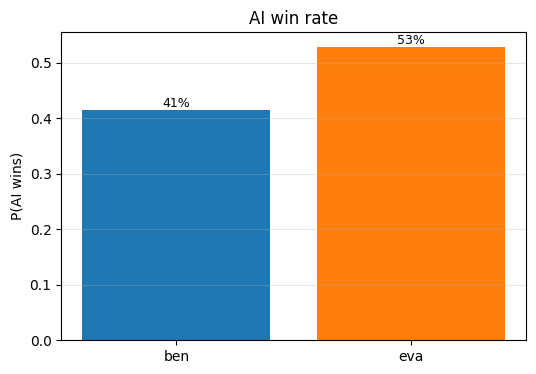
\includegraphics[width=0.75\textwidth]{graphs_objective/winrate_ais.png}
    \caption{Agents win rate in mirror match}
    \label{fig:winrate_ais}
\end{figure}

\begin{figure}[H]
    \centering
    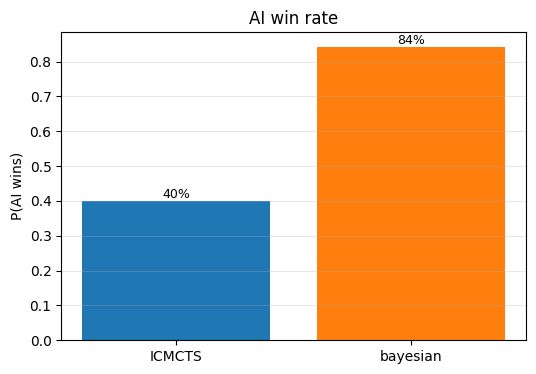
\includegraphics[width=0.75\textwidth]{graphs_objective/winrate_merged.png}
    \caption{Agents win rate against human players}
    \label{fig:winrate_human}
\end{figure}



Despite the substantial difference in win rate, the final hand value each agent reaches remains consistent. In the mirror match, the baseline's final hand value sits around 15, and the Bayesian agent's at around 13 (Figure~\ref{fig:handvalue_ais}), and against human players both agents again finish in a similar range (Figure~\ref{fig:handvalue_human}). This proves how the AI score stays largely stable across both opponents and both testing modes, regardless of the win rate swinging dramatically. This suggests that the limited number of variables and the low uncertainty in Cambio keep the achievable end scores within a narrow band, so that the difference between the agents shows up in who wins far more than in the raw score either one reaches.



\begin{figure}[H]
    \centering
    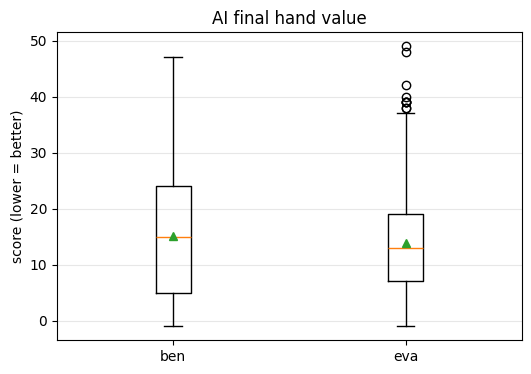
\includegraphics[width=0.75\textwidth]{graphs_objective/hand_value_ais.png}
    \caption{Agents hands average score in mirror match}
    \label{fig:handvalue_ais}
\end{figure}

\begin{figure}[H]
    \centering
    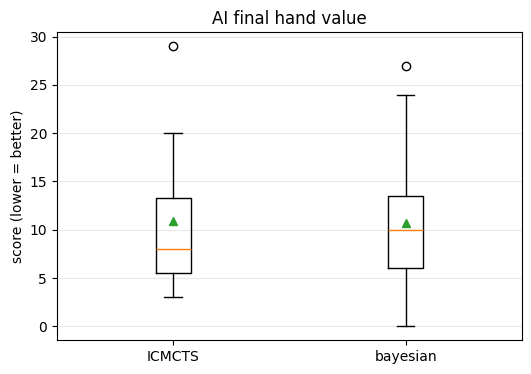
\includegraphics[width=0.75\textwidth]{graphs_objective/hand_value_merged.png}
    \caption{Agents hands average score against human players}
    \label{fig:handvalue_human}
\end{figure}


The score margin between the player and the AI supports the same conclusion. In the mirror match, both agents finish close to level, with the Bayesian agent only slightly above zero (Figure~\ref{fig:score_margin_ais}). Against human players, however, the two agents separate more clearly. The baseline has a median margin of approximately -4, indicating that it finishes slightly behind the human player, while the Bayesian agent has a median margin of around +13, placing it clearly ahead (Figure~\ref{fig:score_margin_human}). As with the win rate, the score margin remains relatively close in the mirror matches but becomes substantially wider against human opponents, while the absolute hand value remains broadly similar. The spikes observed in the Bayesian agent's hand score are also worth noting, as they appear in this figure and throughout the wider analysis. The reason for these spikes is discussed in the discussion section.


\begin{figure}[H]
    \centering
    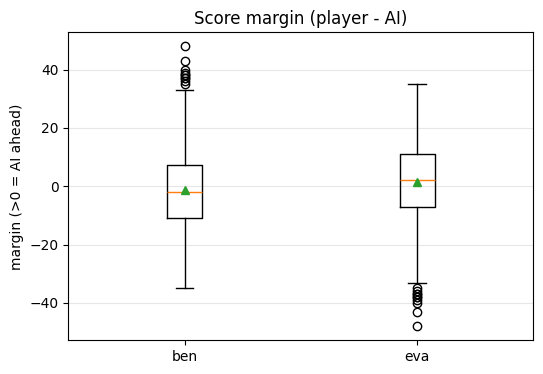
\includegraphics[width=0.75\textwidth]{graphs_objective/score_margin_ais.png}
    \caption{Agents score margin in mirror match}
    \label{fig:score_margin_ais}
\end{figure}

\begin{figure}[H]
    \centering
    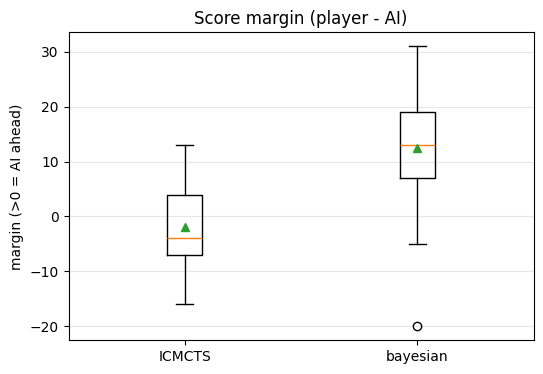
\includegraphics[width=0.75\textwidth]{graphs_objective/score_margin_merged.png}
    \caption{Agents score margin against human players}
    \label{fig:score_margin_human}
\end{figure}

Now after analyzing how each agent plays, evidence most favour the Bayesian agent by a smaller amount. Its swaps are better with an average value change of a swap around -4.6 for the Bayesian agent against -2.4 for the baseline (Figure~\ref{fig:swapquality_human}) against human players, and a -3.5 versus -3.0 in the mirror match(Figure~\ref{fig:swapquality_ais}).Also it draws far fewer penalty cards with a gap of 1.20 versus 0.32 against humans (Figure~\ref{fig:penalties_human}), but not as significant in the mirror match (Figure~\ref{fig:penalties_ais}).

\begin{figure}[H]
    \centering
    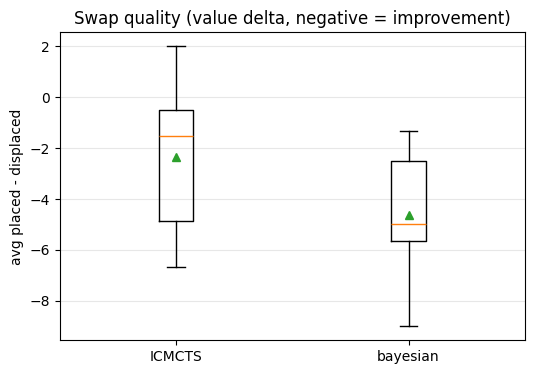
\includegraphics[width=0.75\textwidth]{graphs_objective/swap_quality_merged.png}
    \caption{Agents swap quality against human players}
    \label{fig:swapquality_human}
\end{figure}

\begin{figure}[H]
    \centering
    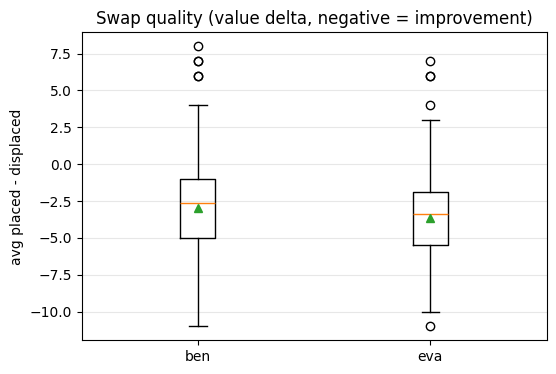
\includegraphics[width=0.75\textwidth]{graphs_objective/swap_quality_ais.png}
    \caption{Agents swap quality in mirror match}
    \label{fig:swapquality_ais}
\end{figure}

\begin{figure}[H]
    \centering
    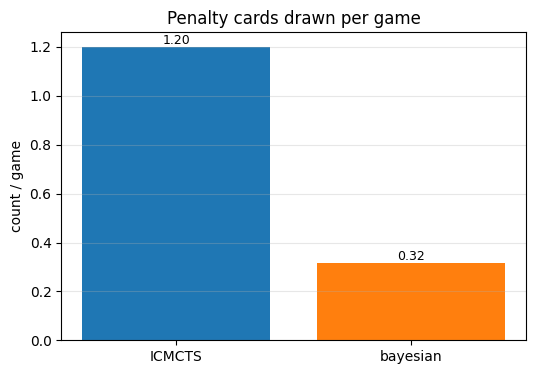
\includegraphics[width=0.75\textwidth]{graphs_objective/penalty_cards_merged.png}
    \caption{Agents penalty cards against human players}
    \label{fig:penalties_human}
\end{figure}

\begin{figure}[H]
    \centering
    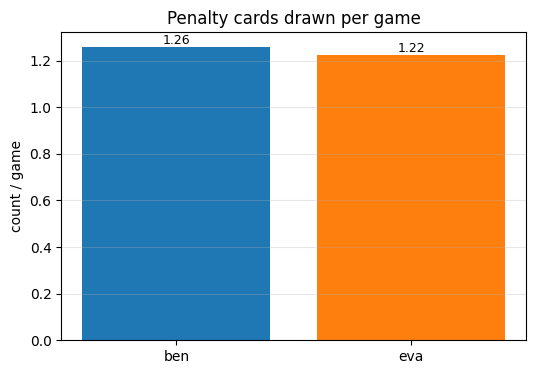
\includegraphics[width=0.75\textwidth]{graphs_objective/penalty_ais.png}
    \caption{Agents penalty cards  in mirror match}
    \label{fig:penalties_ais}
\end{figure}

However, the mean number of the agent's own still-hidden cards per decision is effectively identical, at 1.98 against 1.97 against human players (Figure~\ref{fig:hidden_human}) which suggest that the way both AI improve their own hand does not change at all. For the match hit rate, in the mirror match, Bayesian got a 53\% against the 51\% of the baseline AI, whereas against humans the Bayesian agent is clearly ahead, at 76\% against 55\% (Figure~\ref{fig:hitrate_human}). In the mirror match the successful-match split also differs in kind, with the Bayesian agent matching more often on its own cards and much less on the opponent's (Figure~\ref{fig:matches_ais}).

\begin{figure}[H]
    \centering
    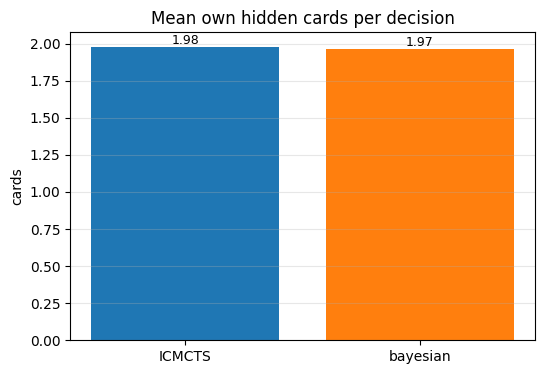
\includegraphics[width=0.75\textwidth]{graphs_objective/hiddeon_own_merged.png}
    \caption{Agents hidden slots against human players}
    \label{fig:hidden_human}
\end{figure}

\begin{figure}[H]
    \centering
    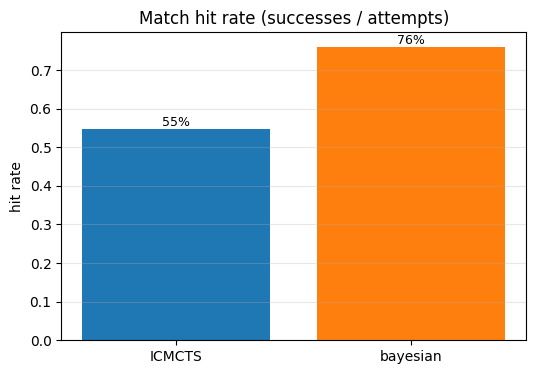
\includegraphics[width=0.75\textwidth]{graphs_objective/match_hit_rate_merged.png}
    \caption{Agents match hit rates against human players}
    \label{fig:hitrate_human}
\end{figure}

\begin{figure}[H]
    \centering
    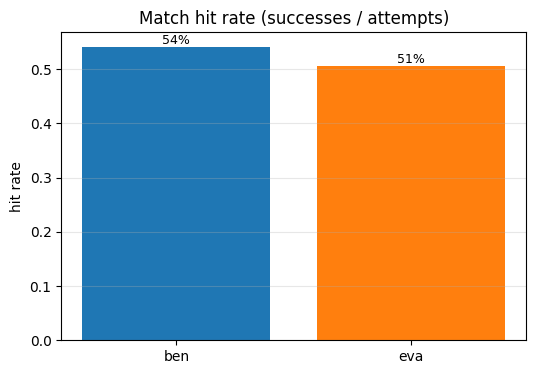
\includegraphics[width=0.75\textwidth]{graphs_objective/match_hite_rate_ais.png}
    \caption{Agents match hit rates in mirror match}
    \label{fig:matches_ais}
\end{figure}

The clearest behavioural difference is in how the two agents end the game. The Bayesian agent calls Cambio earlier and more frequently. In the mirror match, its median call occurs on turn three, compared with turn six for the baseline agent (Figure~\ref{fig:cambio_turn_ais}), and it produces substantially more calls overall. Its accuracy when calling remains high, although it is not higher than the baseline's, as reflected in the baseline being ahead in 143 of 146 calls, while the Bayesian agent was ahead in 295 of 336 calls (Figure~\ref{fig:cambio_ahead_ais}). 

\begin{figure}[H]
    \centering
    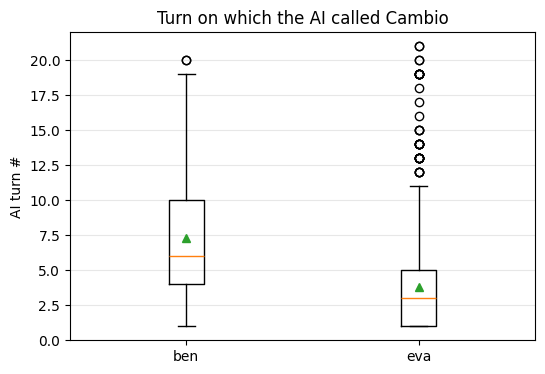
\includegraphics[width=0.75\textwidth]{graphs_objective/cambio_call_ais.png}
    \caption{Agents cambio call turn in mirror match}
    \label{fig:cambio_turn_ais}
\end{figure}

\begin{figure}[H]
    \centering
    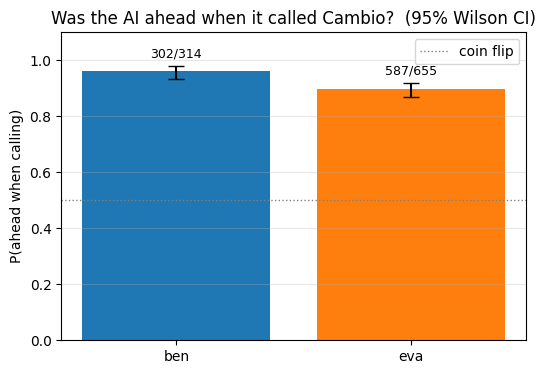
\includegraphics[width=0.75\textwidth]{graphs_objective/cambio_ahead_ias.png}
    \caption{Agents cambio call while being ahead ratio in mirror match}
    \label{fig:cambio_ahead_ais}
\end{figure}

Against human players, the same pattern was observed: the Bayesian agent was ahead in all 16 of its calls, while the baseline was ahead in 5 of 7. These figures should be interpreted cautiously because of the small number of observations (Figure~\ref{fig:cambio_ahead_human}). The per-call guard calibration provides further support for this behaviour, showing that Bayesian calls generally occur above the 0.60 confidence threshold enforced by the guard, with most calls being made when the agent was genuinely ahead (Figure~\ref{fig:guard_cal}).

\begin{figure}[H]
    \centering
    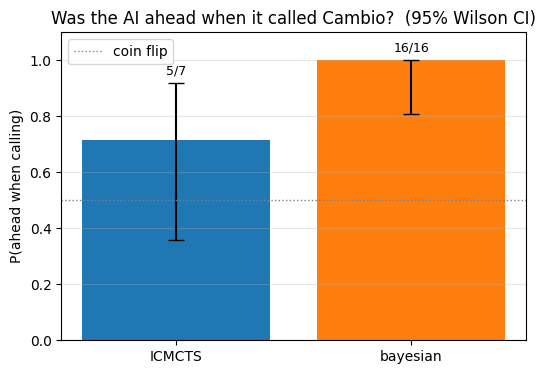
\includegraphics[width=0.75\textwidth]{graphs_objective/cambio_ahead_merged.png}
    \caption{gents cambio call while being ahead ratio against human players}
    \label{fig:cambio_ahead_human}
\end{figure}

\begin{figure}[H]
    \centering
    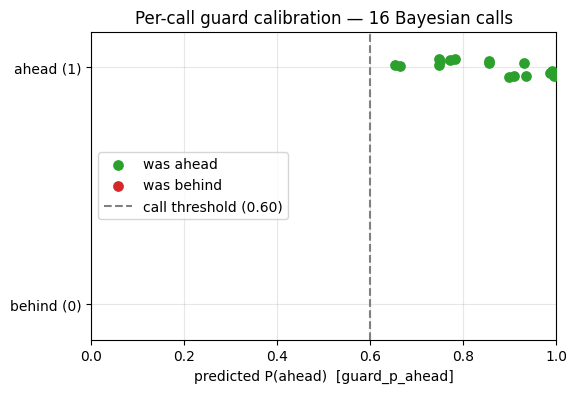
\includegraphics[width=0.75\textwidth]{graphs_objective/guard_calibration_merged.png}
    \caption{Agents cambio guard calibration against human players}
    \label{fig:guard_cal}
\end{figure}

A final metric examines the internal behaviour of the belief layer itself and is available only from the human games because it depends on modelling a distinct opponent. Figure~\ref{fig:belief_tilt} shows the effective tilt applied by the layer to each hidden slot, grouped by the card's true value and separated between opponent slots and the agent's own slots. For opponent slots, the tilt varies with the true card value and shows a weak negative correlation (r=-0.32). Lower-valued cards tend to receive larger positive tilts, while the applied tilt decreases towards zero as the true value increases. The effect is strongest across the low-to-mid value range, although there is considerable variation within each value. For the agent's own slots, the tilt remains effectively zero across all true values. The layer therefore applies very little adjustment to the agent's own cards and instead concentrates its belief updates on opponent slots, which is where the opponent-evidence model is designed to operate.

\begin{figure}[H]
    \centering
    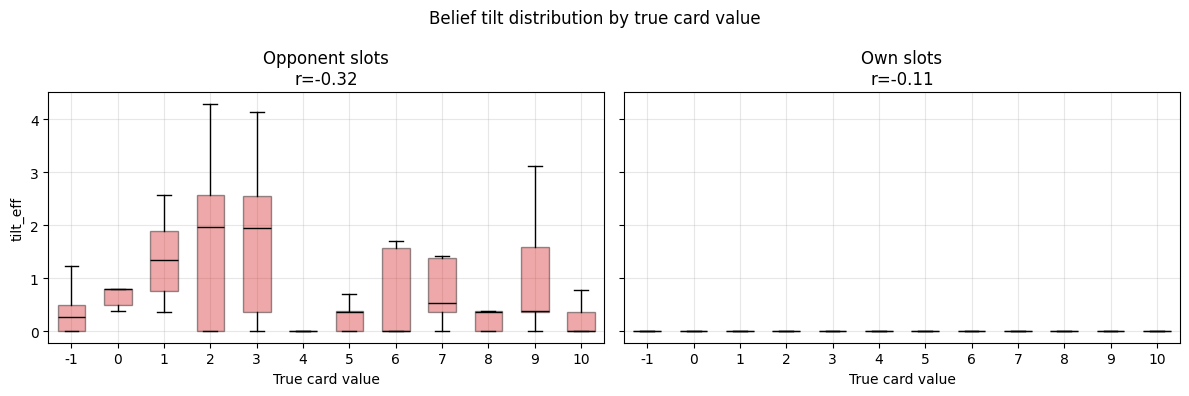
\includegraphics[width=\textwidth]{graphs_objective/belief_distribution_merged.png}
    \caption{Agents belief distribution on hidden cards}
    \label{fig:belief_tilt}
\end{figure}

To validate whether the differences observed between the two agents are statistically significant, a Mann-Whitney U test was performed across every shared metric in the match, call, and belief data. The full output is shown below:

\begin{table}[H]
\centering
\small
\begin{tabular}{llcc}
\hline
\textbf{File} & \textbf{Metric} & \textbf{p-value} & \textbf{Significant} \\
\hline
matches & ai\_win\_rate & 0.0317 & Yes \\
matches & ai\_score & 0.8721 & No \\
matches & player\_score & 0.0005 & Yes \\
matches & ai\_turns & 0.0002 & Yes \\
matches & ai\_swaps & 0.0005 & Yes \\
matches & ai\_discards & 0.0274 & Yes \\
matches & ai\_swap\_value\_delta\_avg & 0.1113 & No \\
matches & ai\_unknown\_swaps & 0.0351 & Yes \\
matches & ai\_hidden\_own\_avg & 1.0000 & No \\
matches & ai\_match\_attempts & 0.0870 & No \\
matches & ai\_match\_success & 0.1108 & No \\
matches & ai\_match\_fail & 0.2278 & No \\
matches & ai\_matches\_on\_own & 0.0184 & Yes \\
matches & ai\_matches\_on\_opponent & 0.2068 & No \\
matches & ai\_penalties & 0.2278 & No \\
matches & ai\_power\_cards\_drawn & 0.0005 & Yes \\
matches & ai\_powers\_played & 0.0030 & Yes \\
matches & ai\_power\_look\_own & 0.0101 & Yes \\
matches & ai\_power\_look\_opp & 0.0631 & No \\
matches & ai\_power\_blind\_swap & 0.2797 & No \\
matches & ai\_power\_look\_swap & 0.5138 & No \\
matches & ai\_decision\_ms\_avg & 0.0000 & Yes \\
calls & cambio\_caller\_turn & 0.0003 & Yes \\
calls & cambio\_ai\_score & 0.9234 & No \\
calls & cambio\_player\_score & 0.0002 & Yes \\
calls & cambio\_caller\_was\_ahead & 0.0601 & No \\
calls & cambio\_ai\_believed\_score & 0.0049 & Yes \\
beliefs & tilt\_raw & 0.0316 & Yes \\
beliefs & tilt\_eff & 0.0000 & Yes \\
beliefs & true\_value & 0.0351 & Yes \\
\hline
\end{tabular}
\caption{Mann-Whitney U test results comparing the baseline and Bayesian agents in games against human players.}
\end{table}

Overall, the results show a statistically significant difference between the two agents: 18 of the 30 metrics fall below the p<0.05 threshold, including win rate, player score, decision time, and the belief-tilt values that the Bayesian model directly influences. In particular, the AI's own score is not significantly different (\(p = 0.8721\)), indicating that the two agents achieve comparable results while differing in how they approach the game, generating different experiences for the opponent. The script used to generate these results can be found in the appendix.

\section{User Study Results}\label{sec:user-study}

The sample was drawn almost entirely from people that activly play video games, with 17 of the 20 reporting that they play video games regularly, while familiarity with card and board games was more mixed. Only 5 of the 20 had played Cambio before, so for most participants the ruleset was new. This context matters for drawing deeper conclusions from the results and understanding players' preference for one AI or the other. 

The central observation is that the two agents were perceived very similarly. Across the six evaluation questions, the distributions of responses for the baseline agent (Ben) and the Bayesian agent (Eva) overlap heavily, and no question shows a marked separation between them. Figure~\ref{fig:enjoyment_ben} and Figure~\ref{fig:enjoyment_eva} plus Figure~\ref{fig:qual_strategy_ben} and Figure~\ref{fig:qual_strategy_eva} illustrate how in both cases the response profiles are close to interchangeable.

\begin{figure}[H]
    \centering
    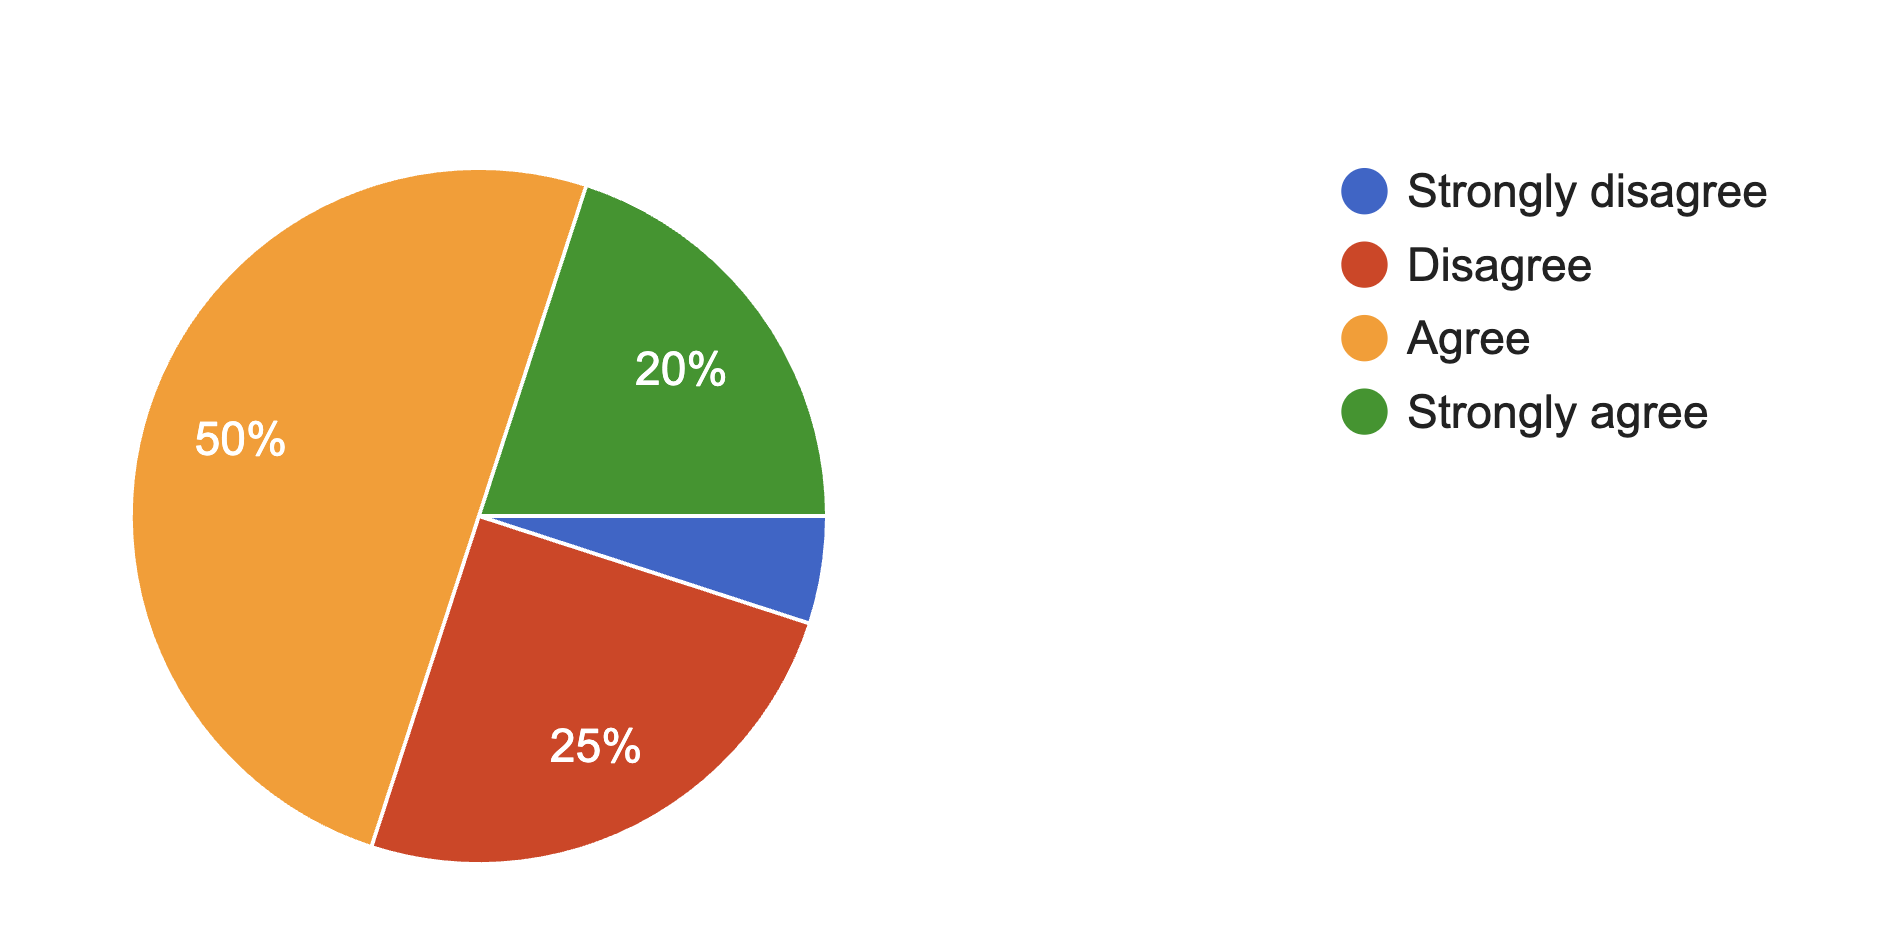
\includegraphics[width=0.8\textwidth]{graph_qualitative/enjoyment_ben.png}
    \caption{Enjoyment ratings for playing against Ben}
    \label{fig:enjoyment_ben}
\end{figure}

\begin{figure}[H]
    \centering
    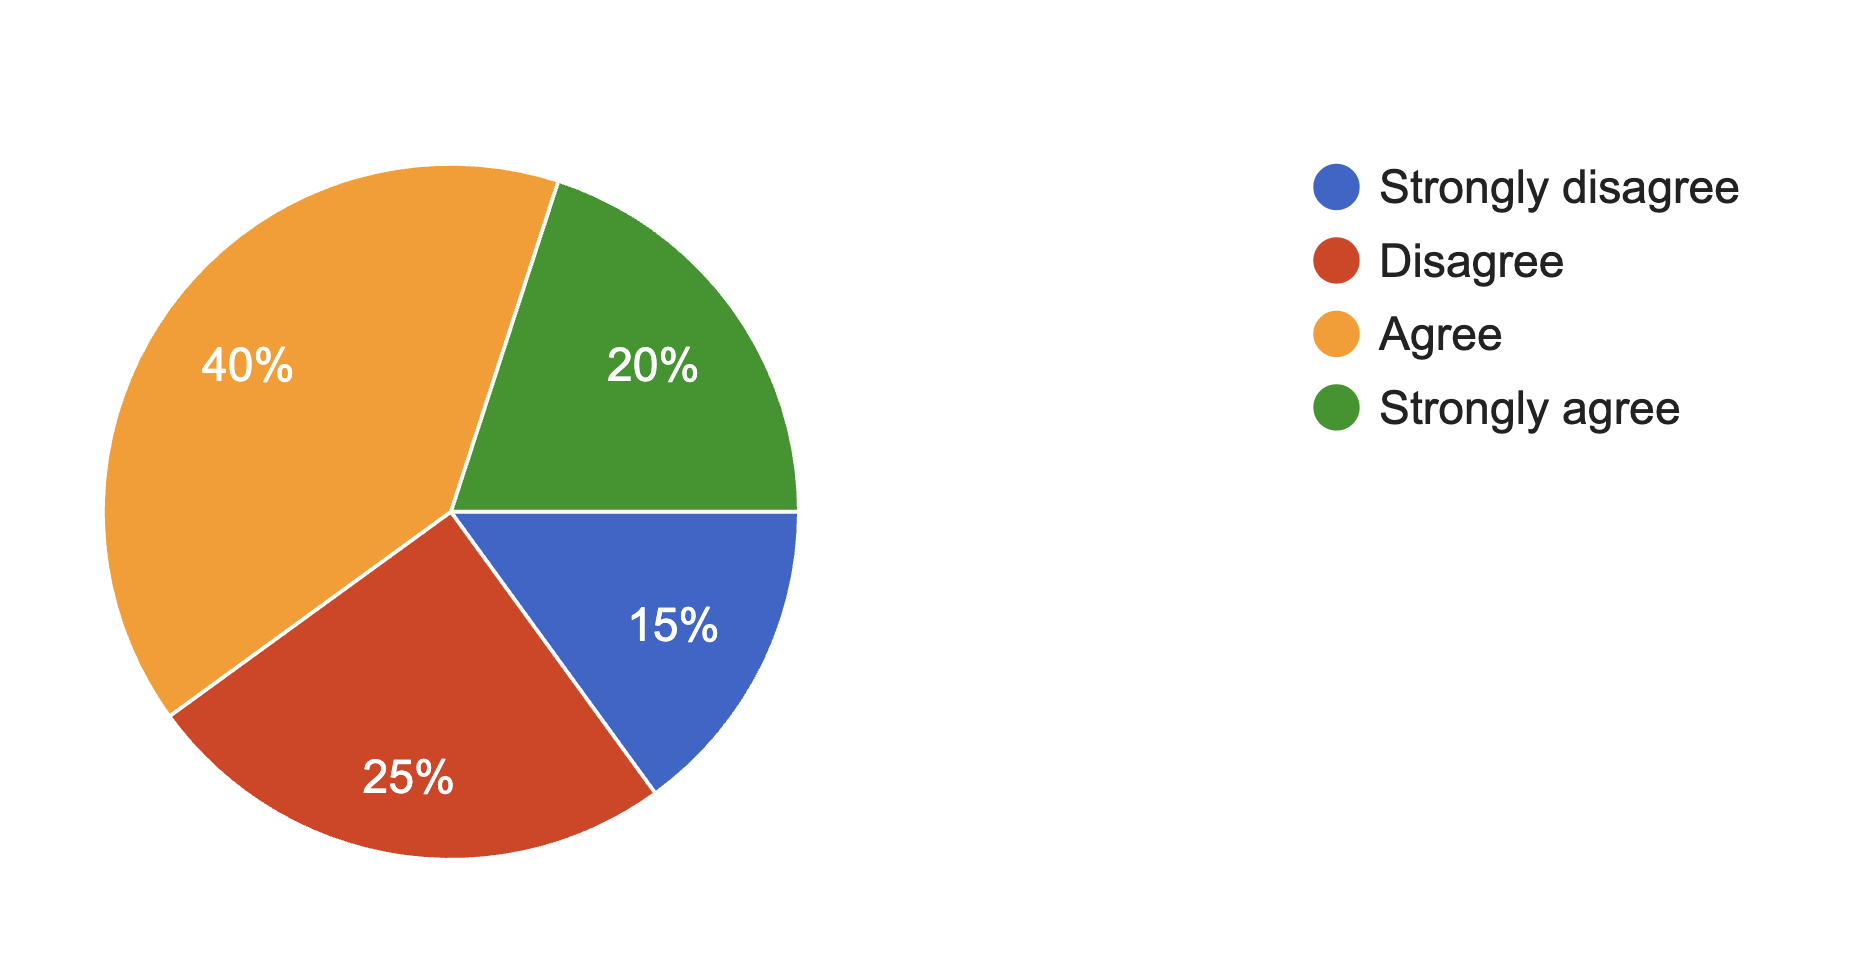
\includegraphics[width=0.8\textwidth]{graph_qualitative/enojoyment_eva.png}
    \caption{Enjoyment ratings for playing against Eva}
    \label{fig:enjoyment_eva}
\end{figure}

\begin{figure}[H]
    \centering
    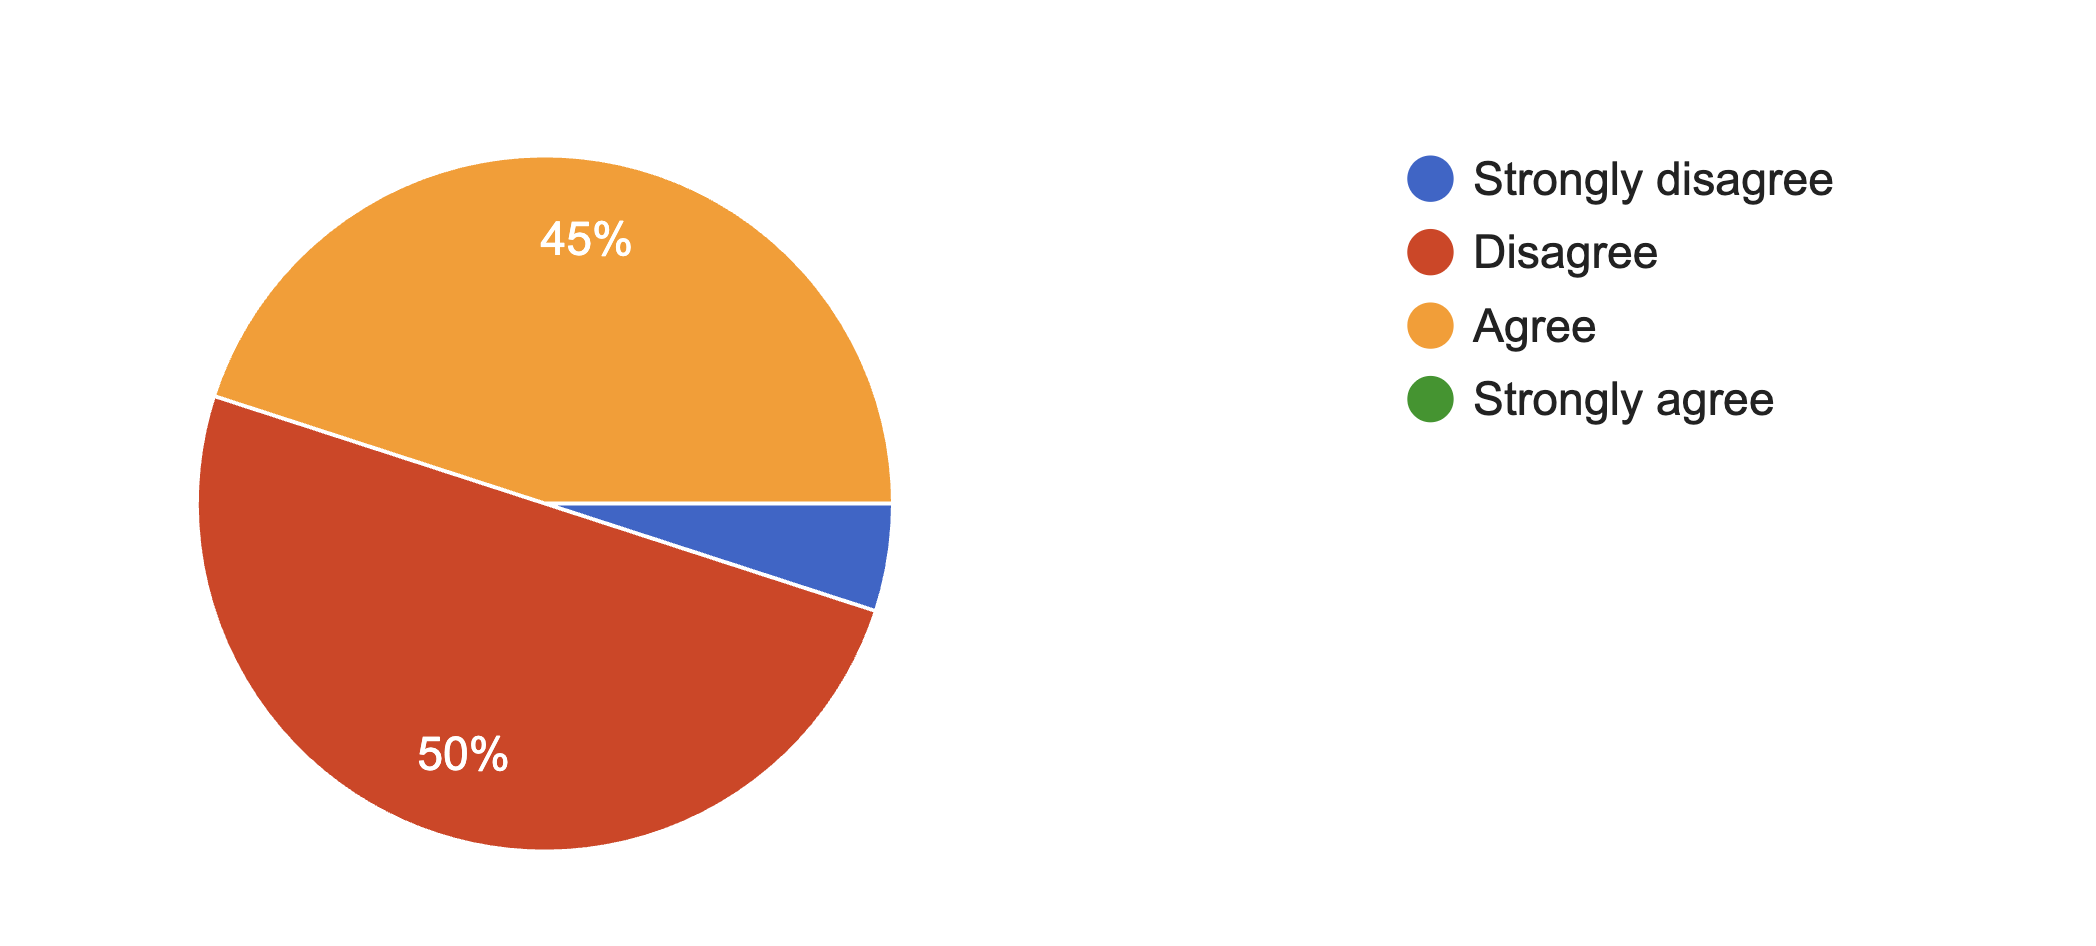
\includegraphics[width=0.9\textwidth]{graph_qualitative/strategy_ben.png}
    \caption{Ratings of Ben’s adaptation to participants’ strategies}
    \label{fig:qual_strategy_ben}
\end{figure}

\begin{figure}[H]
    \centering
    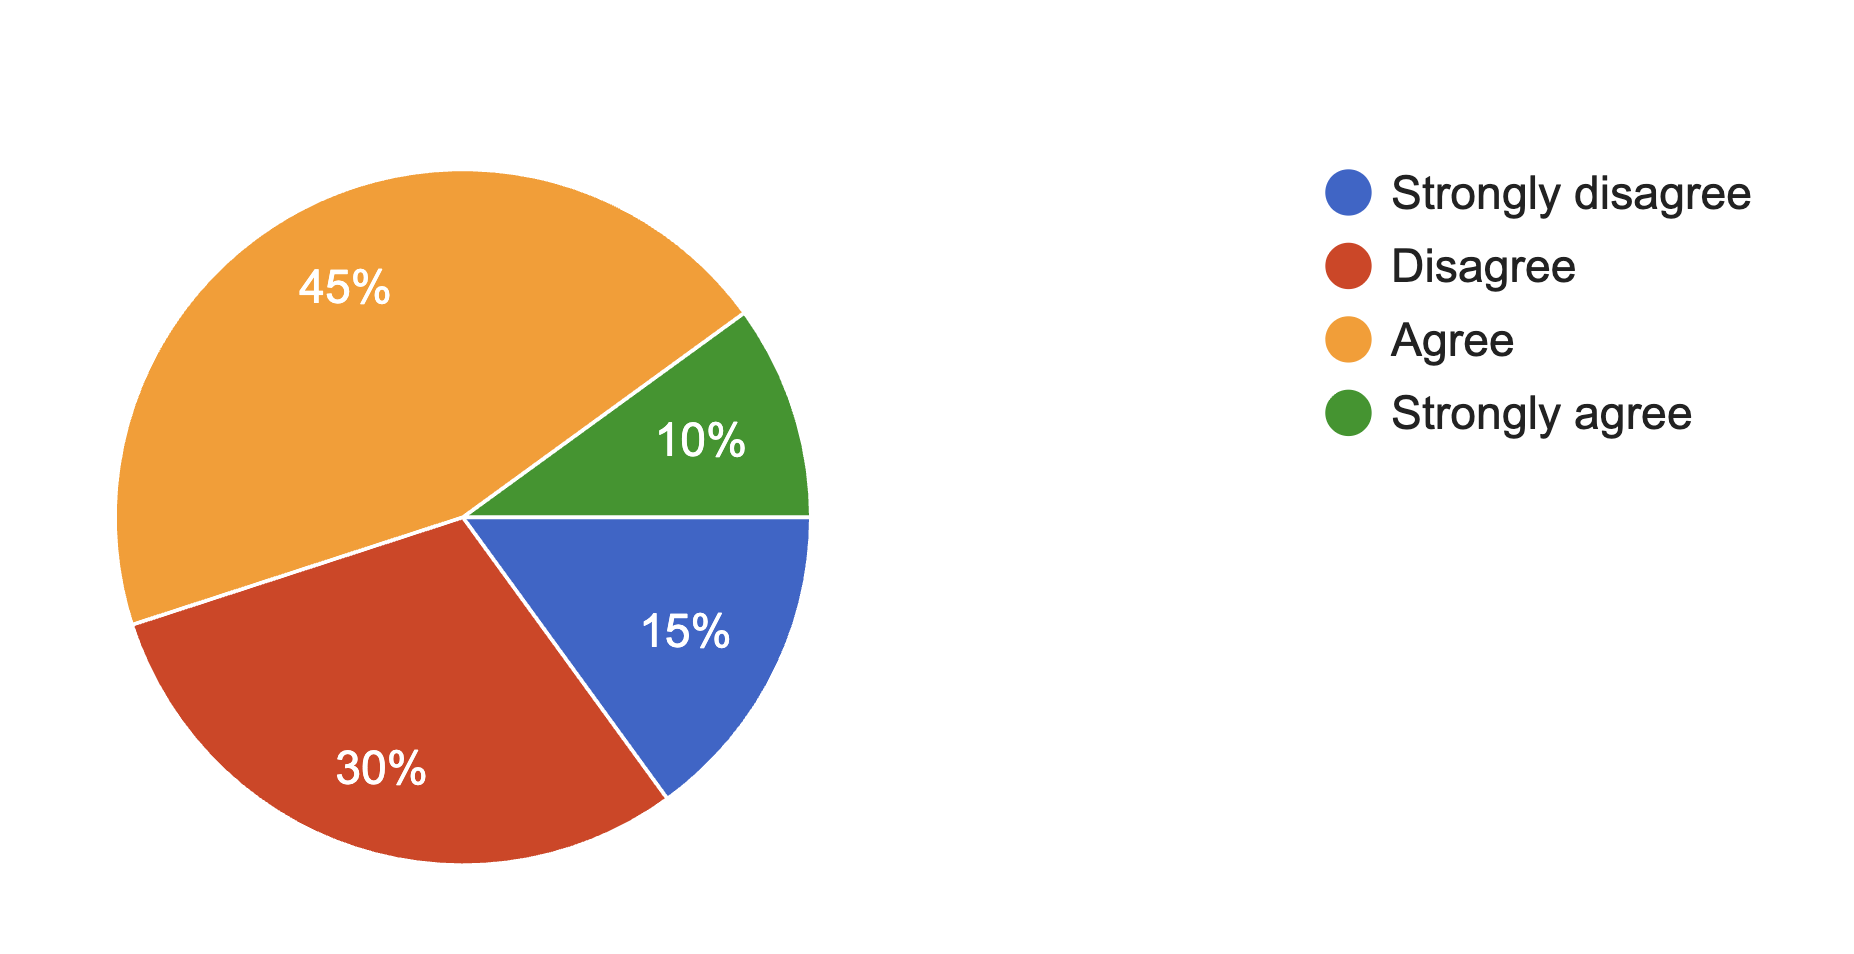
\includegraphics[width=0.8\textwidth]{graph_qualitative/strategy_eva.png}
    \caption{Ratings of Eva’s adaptation to participants’ strategies}
    \label{fig:qual_strategy_eva}
\end{figure}

To confirm that this apparent similarity is accurate, each Likert item was compared between the two agents using a Wilcoxon signed-rank test. The script used to perform these tests can be found in the Appendix. The results were as follows:

\begin{itemize}
    \item \textbf{Enjoyment:} No statistically significant difference between Ben and Eva ($p = 0.294$).
    \item \textbf{Adjusted strategy:} No statistically significant difference between Ben and Eva ($p = 0.623$).
    \item \textbf{Predictability:} No statistically significant difference between Ben and Eva ($p = 0.714$).
    \item \textbf{Had a strategy:} No statistically significant difference between Ben and Eva ($p = 0.354$).
    \item \textbf{Took too long:} No statistically significant difference between Ben and Eva ($p = 0.179$).
\end{itemize}

None of the five items returned a statistically significant difference between the two agents.

The final question asked participants which agent they found more interesting and fun to play against. The Bayesian agent was preferred by 8 participants and the baseline by 7, with the remaining 5 neutral (Figure~\ref{fig:qual_preference}). This is a one-vote margin in the Bayesian agent's favour; therefore, it does not represent a meaningful difference.

\begin{figure}[H]
    \centering
    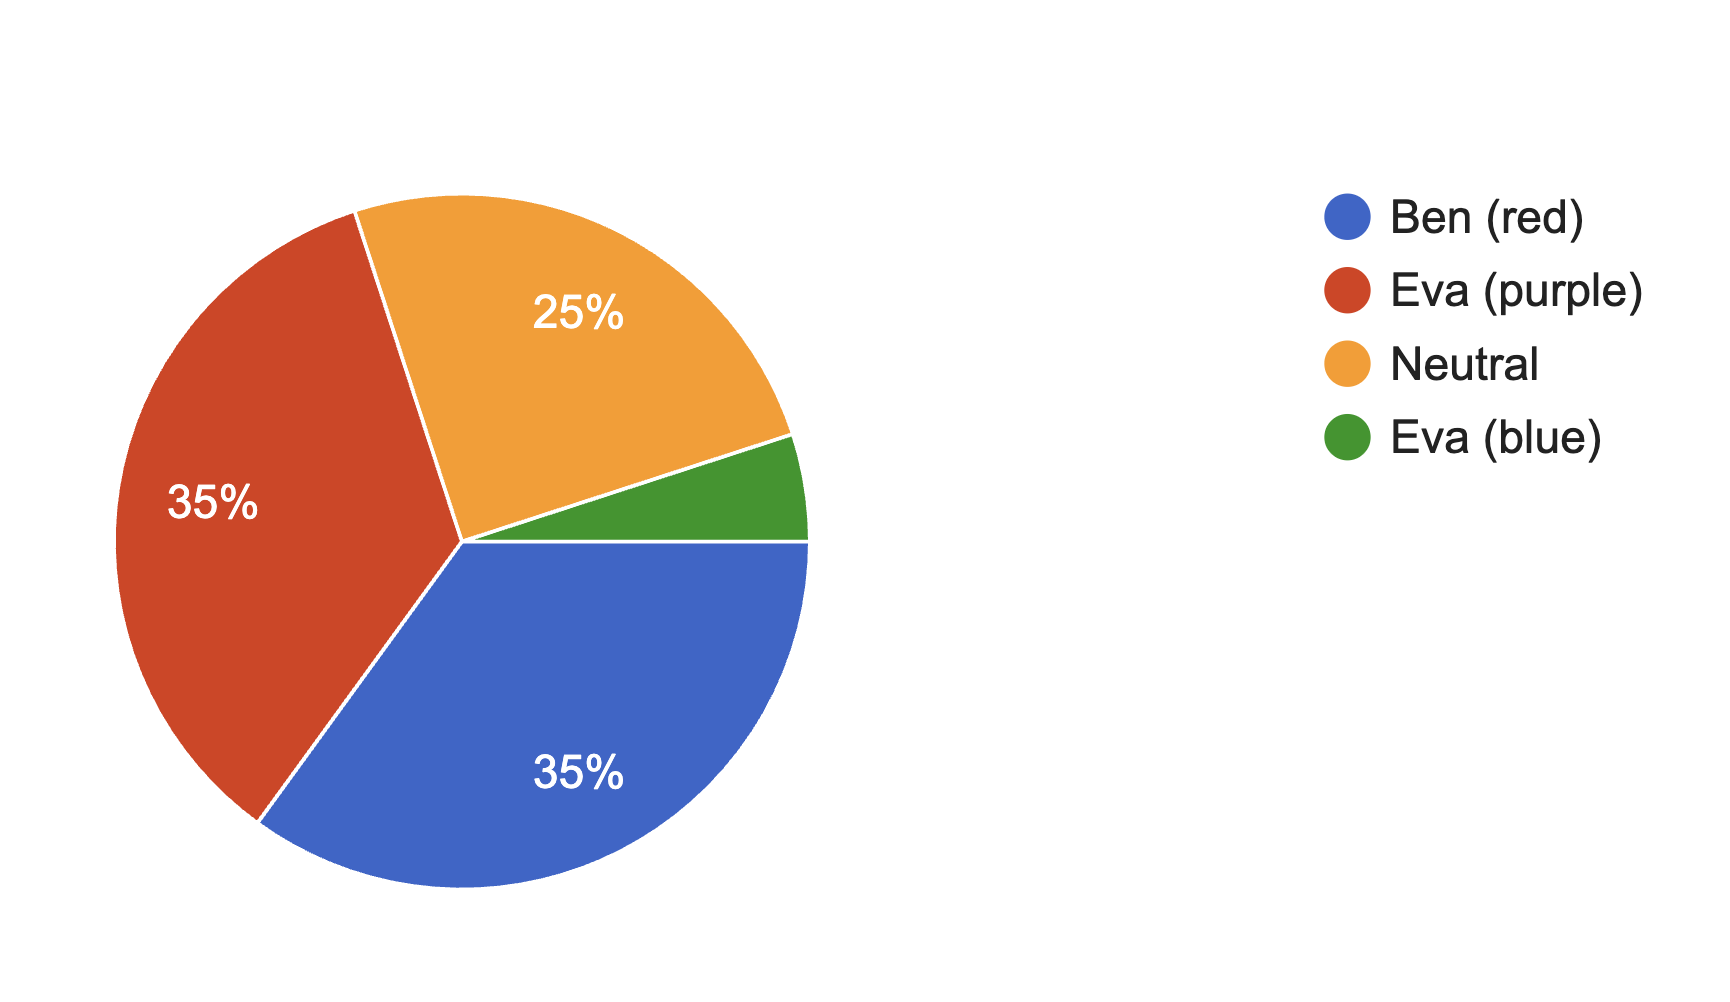
\includegraphics[width=0.8\textwidth]{graph_qualitative/ai_preference.png}
    \caption{Participants' preference for the more enjoyable AI agent}
    \label{fig:qual_preference}
\end{figure}

\section{Computational Performance}
\label{sec:comp-performance}

The only computational cost of interest is the time each agent takes to make a decision, measured as the mean wall-clock time of its tree search per game across the 400 games. The baseline agent averaged 67\,ms per decision and the Bayesian agent 84\,ms (Figure~\ref{fig:computational_performance}). The belief layer added roughly 17\,ms on top of the search, an overhead that is negligible in the context of a turn-based card game where the agent is not competing for a real-time frame budget. 

\begin{figure}[H]
    \centering
    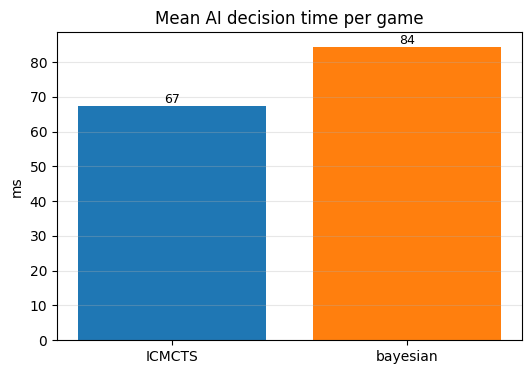
\includegraphics[width=0.75\textwidth]{graphs_objective/decision_time_merged.png}
    \caption{Agents mean decision time per game}
    \label{fig:computational_performance}
\end{figure}

%===========================================================================
%  CHAPTER 6 -- DISCUSSION
%============================================================================

\chapter{Discussion}
\label{chap:discussion}

The results reveal a disagreement between player perceptions and the recorded game outcomes. The questionnaire responses show no significant difference in how the two agents were perceived, with a distribution of 40\% of the votes for Eva (Bayesian agent), 35\% towards Ben (baseline ISMCTS) and 25\% as neutral. The quantitative results, however, do not support the same conclusion. Across the games played against humans, the Bayesian agent outperforms the baseline. The 1000-game mirror match shows the same ordering with much greater statistical confidence, with the win rate increasing from 41\% to 53\%. This chapter argues that this apparent contradiction does not indicate that the belief layer has no effect, but instead results from the conditions under which the human data was collected.

The first and most important of those conditions is that the majority of playtesters had never played Cambio before, which inevitably introduces a layer of friction since a player meeting the game for the first time is simultaneously learning the rules and forming a judgement of the opponent, and the opponent they happened to face first was rated against a background of not yet understanding the game and how it should be played optimally. It was observed that this learning process depresses the enjoyment attributed to the first agent regardless of which agent it was, and because the order in which the two agents were presented was randomised, that penalty falls roughly evenly on Ben and Eva. The lack of a clear difference in player perceptions is likely because the variation introduced by players learning the game covered the differences between the two agents. When the analysis is restricted to games involving players who already understood Cambio, Eva still retains an advantage, although it is more subtle than the headline figures suggest, as it can be seen in Figure~\ref{fig:playtest_winrate}.

\begin{figure}[H]
    \centering
    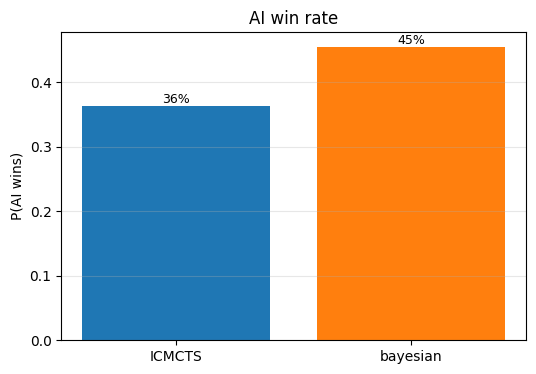
\includegraphics[width=0.75\textwidth]{graphs_objective/playtest_winrate.png}
    \caption{Play tester win rate}
    \label{fig:playtest_winrate}
\end{figure}

Another condition that affected the perception of the players with the AI was that each action the agents took was written to a text log and shown to the player as raw text, rather than visually in the play area. In addition, the pace at which those actions were produced was often faster than a player could follow by reading. This made players miss what had happened; for example, an agent might use a card power to swap a card, and the player would go on to attempt a match without realising that it was swapped or make a decision based on a board state that no longer existed. This frustration from the players attached itself to whichever agent they were playing against. This is a limitation of the measurement instrument rather than a property of the agents themselves, and it is a further reason why the perceived difference between them was compressed toward nothing even as their measured behaviour diverged.

That divergence can be seen in how the two agents decide to end a game. Ben calls Cambio based on a fixed threshold. In contrast, Eva calls whenever she believes her own hand to be lower than her opponent's, and this difference in mechanism produces a significantly more aggressive play style. Crucially, this aggression is exactly an output expected from the design implemented, as she remains ahead at the moment of calling in the large majority of cases, a rate well above chance, which shows the earlier calls are grounded in the belief state and not uninformed gambles. The trade-off is visible in the guard calibration, where Eva's willingness to call admits a cluster of calls made from behind that Ben's more conservative fixed style rarely does, as it is almost always ahead when calling. Still, he takes several more turns to get there. This is precisely the profile the literature associates with a more engaging opponent: one whose play is confident and reasoned but not infallible, rather than one that is cautious to the point of being predictable.

This is also the source of the score spikes noted in Section~\ref{sec:ai-analysis} (Figure~\ref{fig:score_margin_ais}). Because Eva's decision to call rests on a belief rather than on certainty, a call founded on an inaccurate belief occasionally ends the game while she is in fact behind, leaving her with a high final hand that registers as an outlier. The spikes are therefore not noise but the visible cost of belief-driven calling.

The player reactions divide along exactly the fault line this aggression creates based on their experience with the game. Players new to Cambio tended to read Eva's early, frequent calls not as skilful but as erratic behaviour, in part because the calls cut the games short, which doesn't let them keep playing and learn the game.
\begin{quote}
\textit{``Ben is better definitely, Eva is way too hard, she plays too fast. Ben felt balanced''} \\
\hfill --- Play tester \emph{1}
\end{quote}
Experienced players by contrast tended to value the very thing the newer players disliked, describing Eva's playstyle as a more varied and interesting challenge.
\begin{quote}
\textit{``Eva was less predictable, so it was more fun to me. I feel it was harder to like guess what she was gonna do, which made it more fun and challenging. Ben became predictable, so yeah.''} \\
\hfill --- Play tester \emph{2} 
\end{quote}

The clearest sign observed during playtest sessions is that some testers changed their own behaviour in response, beginning to call Cambio earlier themselves to get ahead of Eva's aggression. Although the following quotation does not state this interpretation explicitly, it can be understood as reflecting such an adaptation.
\begin{quote}
\textit{``Ben because I felt I had a chance to win. Didn't enjoy playing against Eva she was too difficult. I felt I was in a race to call cambio.''} \\
\hfill --- Play tester \emph{3}
\end{quote}

Another observation worth stating is that the missed matches produced by the interface helped inexperienced players stay competitive, since plays they failed to register were also plays they were not punished for. But the same gap between what the agent did and what the player perceived meant that Eva's occasional weak decisions based on acting on an uncertain belief were not read as human-like fallibility at all. They were read as stupidity: not an agent that plays well, and not an agent that plays like a person who sometimes errs, but an agent that appears not to realise it is making a mistake.

This is the sharpest lesson of the study since it exposes a gap between design intent and player reading. The belief layer does produce measurably different hidden-slot decisions, but without any expressive feedback to communicate that these choices are deliberate, the behaviour reads as randomness rather than as reasoning; this is expanded in the future work section.

Taken together, these threads answer the research question, and the answer is a qualified no. The question was whether integrating the Bayesian opponent-modelling layer influences player-perceived opponent quality and difficulty, and on the evidence of the questionnaire it does not: players reported no significant difference between the two agents. That negative result, however, sits on top of a clearly positive one that the Bayesian layer does produce a stronger and more adaptive agent, and among the players who already knew Cambio, that improvement was both felt and, in some cases, responded to. The reason the improvement did not surface as a perceived difference across the whole group is that inexperienced players judged Eva while still learning the game, and an interface too fast and too sparse to let her reasoning be seen. This distinction between what was built and what was perceived, and what it would take to close the gap between them, is taken up in the chapters that follow.

%===========================================================================
%  CHAPTER 7 -- CONCLUSION AND FUTURE WORK
%============================================================================
\chapter{Conclusion and Future Work}\label{chap:conclusion}
\section{Conclusion}

This dissertation’s primary goal is to answer whether integrating an adaptive Bayesian
opponent-modelling layer into a static ISMCTS agent influences player-perceived
opponent quality and difficulty within the context of the card game Cambio. To answer this, the standard
uniform determinization of ISMCTS was replaced with a belief-weighted sampler driven by
an opponent-evidence model, following the theory behind Bayes ' theorem. The search itself was left unchanged, so that any measured difference between the two
agents could be attributed to the belief machinery alone.

The questionnaire results show no statistically significant difference between the baseline agent, Ben, and the Bayesian variant, Eva. Based on player perception alone, the belief layer therefore did not clearly change how the opponent was experienced across the full participant group. This negative result, however, exists alongside a clear positive result, which is that the Bayesian layer produces a measurably different and stronger agent. It wins more often in both mirror matches and games against human players, swaps more efficiently, draws fewer penalties, and ends games using a reasoned, distribution-based call rather than a fixed cap, which adds variety to the matches. These changes also come at negligible computational cost. Among participants who already understood Cambio, the difference was more apparent and, in some cases, affected their responses. The most likely reason this difference did not emerge across the full sample is the set of conditions under which the human data was collected, which is addressed in the future work section.

Taken together, the Bayesian layer appears to add a distinct playstyle that varies the
behaviour of standard ISMCTS while remaining slightly stronger objectively in this
context, which makes it an overall better agent in the context of this dissertation. Cambio is a small game with little hidden information, so the ceiling for what such a layer can demonstrate here is limited; its true impact would need to be measured
in larger hidden-information games, with longer horizons and more players, before strong
claims could be made. Even within these constraints, however, belief-weighted
determinization driven by observed opponent behaviour looks like a promising and
 interesting direction for building adaptive game AI, and one worth developing
further.


\section{Future Work}

The study produced a clear result about the agents' behaviour but a much weaker one about
how that behaviour was perceived, and most of the future work follows from closing that
gap. The directions below are ordered from the changes that would most improve the
measurement to the changes that would most extend the contribution itself.

\subsection{Improving the Study Design}

Two aspects of the study introduced bias that was not anticipated beforehand and that a future version should remove. First, the  questionnaire never recorded which agent each participant played first. Because
most testers were playing Cambio for the first time, the opponent they faced
first was judged while they were still learning the rules, which depressed its ratings
regardless of which agent it was. Adding a single question that records the order of play
would let this learning penalty be measured and controlled for. Second, the sample was small and largely unfamiliar with the game. While 400 matches is a really decent number of data samples, especially taking into account the time given for this dissertation, a larger cohort, deliberately including more players who already know Cambio, would reduce the
noise that first-time learning introduced and give the perception data enough power to
detect a difference the behavioural data shows is really there.


\subsection{Communicating the Agent's Actions}

The single change that would have had more impact on how the AI was perceived is to add a layer of visual polish and feedback. In the current build, each power, swap, and decision the agent made was written to a text log rather
than shown in the play area, and often faster than a player could read. The majority of
playtesters reported that this made the game hard to follow; there was a point at which
they felt lost and would call Cambio just to end a turn they no longer understood.
Replacing the log with visual feedback, with the actual cards moving in the scene as
powers and swaps resolve, would let players concentrate on the game itself instead of
trying to follow it with the text logs, and would give them a far better basis for judging the
opponent. It is worth noting that some difficulty in tracking is inherent to Cambio, since forgetting one's own or the opponent's cards is part of the game, and this is precisely why the agent was allowed to make mistakes; but the text log amplified that difficulty well beyond what the game itself imposes.

\subsection{Making Mistakes Read as Human}

The agent's capacity for mistakes helped inexperienced players to play longer and sneak some wins, but over time it read as a negative signal because the agent gives no sign of recognising that a
belief-driven choice went wrong, making its behaviour come across as robotic and dumb rather than as
human fallibility. One way to close this gap can be through expressive feedback:
short comments that convey emotion or personality at the moment of a negative match attempt,
such as "What?!" or "Wasn't this an eight?" could make the mistake read as a human error
a player can empathise with rather than as a machine failing silently. Another way could be a
light Dynamic Difficulty Adjustment layer that monitors how well the human is doing and,
when the player is winning by a comfortable margin, disables the mistake-prone behaviour
through a flag. This is admittedly a hard-coded intervention that removes some of the
agent's autonomy, but in a game as short as Cambio it would make the opponent feel
noticeably smarter and more responsive at the moments where it matters most.

\subsection{Scaling to Larger Hidden-Information Games}

Finally, Cambio's small state space limits what this layer can demonstrate since it is not being exposed to enough stress. At any moment, there are usually only around six hidden cards, two on the player's side and four on the opponent's, and while this number shifts as powers and swaps reveal and move cards, it
rarely grows beyond that. Games also tend to end quickly. In such a small space it is easy
for a player to mistake a strong-looking baseline play for a deliberate strategy when it
was effectively random, simply because the odds of a good random outcome are high when so
few cards are in play. A more demanding test would move the layer into a game with a longer
horizon, giving the agent time to accumulate evidence and refine its beliefs and giving the
player time to notice that adaptation. Cambio can also be played with more than two players,
so another route could be to place three Bayesian agents against a single human; the way
this multiplies the hidden state and the interacting beliefs could either reveal the layer's
true strength or expose weaknesses that the two-player setting never stressed.


%===========================================================================
%  REFERENCES
%============================================================================
\printbibliography[heading=bibintoc]

%===========================================================================
%  BACK MATTER
%============================================================================

\chapter*{Acknowledgment of AI Tools}
\addcontentsline{toc}{chapter}{Acknowledgment of AI Tools}

This section declares the generative AI tools used during the preparation of this dissertation, together with the purpose for which each was used.

\begin{itemize}
  \item \textbf{Grammarly:} Used for grammar, spelling, and vocabulary checking throughout the written document.
  \item \textbf{GPT-5.6 Luna (OpenAI):} Used for grammar checking, guidance on document structure, and LaTeX formatting support.
  \item \textbf{Claude Opus 4.8 (Anthropic):} Used for code debugging, assistance in producing the plots and graphs presented in the results, and building debugging tools used to inspect and test the AI agents' decision-making.
\end{itemize}

%===========================================================================
%  APPENDICES
%============================================================================
\begin{appendices}

\chapter{Project Materials and Reproducibility}
\label{app:materials}

All materials required to replicate the results presented in this dissertation are publicly available. The repository contains the complete Unity project source, a standalone Windows build together with play-testing instructions, all
raw data collected during the study, and a link to the Google Colab notebooks used to perform the statistical analysis and generate the graphs.

The materials can be accessed at the following address:

\begin{center}
\url{https://github.com/PabloGP88/bayesian-ismcts-cambio}
\end{center}

\noindent If the link above is not clickable, the address can be typed manually.

\chapter{Statistical Analysis Scripts}
\label{app:scripts}

This appendix reproduces the two Python scripts used to produce the statistical
results reported in Chapter~\ref{chap:results}. Both were run in Google Colab. 

\section*{Wilcoxon Signed-Rank Test}  

\begin{lstlisting}[style=python]
# Wilcoxon Signed-Rank Tests

import pandas as pd
import numpy as np
from scipy.stats import wilcoxon
from google.colab import files


# Upload and load the CSV

uploaded = files.upload()
filename = list(uploaded.keys())[0]
df = pd.read_csv(filename)

print("Data loaded successfully.\n")
display(df.head())


# Convert Likert responses to numbers (case/space tolerant)

likert_map = {
    "strongly disagree": 1,
    "disagree": 2,
    "neutral": 3,
    "agree": 4,
    "strongly agree": 5,
}

def convert_column(col):
    mapped = col.astype(str).str.strip().str.lower().map(likert_map)
    # keep original value where it wasn't a Likert label
    return mapped.where(mapped.notna(), col)

df_numeric = df.apply(convert_column)

print("\nConverted data:")
display(df_numeric.head())


# 3. Comparisons - matched by KEY PHRASE, not full header

comparisons = {
    "Enjoyment":         "enjoy playing against",
    "Adjusted strategy": "adjusted his strategy",
    "Predictability":    "feel predictable",
    "Had a strategy":    "had a strategy",
    "Took too long":     "taking to long",
}

def find_column(df, phrase, name):
    """Find the one column containing both `phrase` and the person's `name`."""
    phrase, name = phrase.lower(), name.lower()
    matches = [c for c in df.columns
               if phrase in c.lower() and name in c.lower()]
    if len(matches) == 1:
        return matches[0]
    elif not matches:
        raise KeyError(f"No column found for '{phrase}' + '{name}'")
    else:
        print(f"[!] Multiple matches for '{phrase}' + '{name}': {matches}. "
              f"Using the first.")
        return matches[0]


# Wilcoxon signed-rank tests

results = []

for measure, phrase in comparisons.items():

    try:
        ben_col = find_column(df_numeric, phrase, "Ben")
        eva_col = find_column(df_numeric, phrase, "Eva")
    except KeyError as e:
        print(f"Skipping '{measure}': {e}")
        continue

    ben = pd.to_numeric(df_numeric[ben_col], errors="coerce")
    eva = pd.to_numeric(df_numeric[eva_col], errors="coerce")

    valid = ben.notna() & eva.notna()
    ben, eva = ben[valid], eva[valid]

    if len(ben) == 0:
        print(f"Skipping '{measure}': no valid paired responses.")
        continue
    if (eva - ben).abs().sum() == 0:
        print(f"Skipping '{measure}': all differences are zero.")
        continue

    statistic, p_value = wilcoxon(eva, ben)

    results.append({
        "Measure": measure,
        "N": len(ben),
        "Ben Median": ben.median(),
        "Eva Median": eva.median(),
        "Wilcoxon W": statistic,
        "p-value": p_value,
        "Significant (p < .05)": "Yes" if p_value < 0.05 else "No",
    })


# Display results

if not results:
    print("\nNo tests could be run - check the phrases in `comparisons`.")
else:
    results_df = pd.DataFrame(results)
    print("\nWilcoxon Signed-Rank Test Results:")
    display(results_df)

    print("\nInterpretation:")
    print("A p-value below 0.05 indicates a statistically significant")
    print("difference between participants' ratings of Eva and Ben.\n")

    for _, row in results_df.iterrows():
        verdict = "SIGNIFICANT" if row["p-value"] < 0.05 else "NO significant"
        print(f"{row['Measure']}: {verdict} difference "
              f"(p = {row['p-value']:.3f})")
\end{lstlisting}

\section*{Mann--Whitney U Test}

\begin{lstlisting}[style=python]
import pandas as pd
import numpy as np
from scipy.stats import mannwhitneyu, fisher_exact
from google.colab import files

uploaded = files.upload()


data = {"matches": {}, "calls": {}, "beliefs": {}}
for fname in uploaded:
    low = fname.lower()
    ftype = next((t for t in data if t in low), None)
    cond = "baseline" if "baseline" in low else "bayesian" if "bayesian" in low else None
    if ftype and cond:
        data[ftype][cond] = pd.read_csv(fname)


EXCLUDE = {"match_index", "bayesian_on", "ply", "ai_turn",
           "is_opponent_slot", "opp_knows", "completed"}

rows = []

for ftype, pair in data.items():
    if "baseline" not in pair or "bayesian" not in pair:
        continue
    base_df, bayes_df = pair["baseline"], pair["bayesian"]

    # Win rate via Fisher's exact test
    if ftype == "matches" and "winner" in base_df.columns:
        def wins(df):
            w = df["winner"].astype(str).str.strip().str.lower()
            return (w == "ai").sum(), (w != "ai").sum()
        yw, yl = wins(bayes_df)
        bw, bl = wins(base_df)
        _, p = fisher_exact([[yw, yl], [bw, bl]])
        rows.append([ftype, "ai_win_rate", round(p, 4), "Yes" if p < 0.05 else "No"])


    common = [c for c in base_df.columns
              if c in bayes_df.columns and c not in EXCLUDE]
    for col in common:
        base = pd.to_numeric(base_df[col], errors="coerce").dropna()
        bayes = pd.to_numeric(bayes_df[col], errors="coerce").dropna()
        if len(base) == 0 or len(bayes) == 0:
            continue
        if base.nunique() == 1 and bayes.nunique() == 1 and base.iloc[0] == bayes.iloc[0]:
            continue
        try:
            _, p = mannwhitneyu(bayes, base, alternative="two-sided")
        except ValueError:
            continue
        rows.append([ftype, col, round(p, 4), "Yes" if p < 0.05 else "No"])

results = pd.DataFrame(rows, columns=["File", "Metric", "p-value", "Significant"])
display(results)
\end{lstlisting}

\chapter{Questionnaire}
\label{app:questionnaire}

\section*{Part A: Participant background}
\begin{enumerate}
  \item Do you play video games?\\
        \emph{(Yes, regularly / Occasionally / Rarely / No)}
  \item Do you play card or board games?\\
        \emph{(Yes, regularly / Occasionally / Rarely / No)}
  \item Have you played card games similar to Golf, Skyjo, or Poker?\\
        \emph{(Yes / No)}
  \item Have you played Cambio before?\\
        \emph{(Yes / No)}
  \item Please select your age group.\\
        \emph{(18--24 / 25--34 / 35--49 / 50+)}
\end{enumerate}

\section*{Part B: Agent evaluation}

\begin{enumerate}
  \item Did you enjoy playing against (agent)?
  \item Do you feel (agent) adjusted its strategy based on how you were playing?
  \item Did (agent) feel predictable at any moment during the match?
  \item Did (agent) feel like it had a strategy?
  \item Did (agent) respond differently when you used special cards such as peek or swap?\\
        \emph{(Yes / No / Neutral)}
  \item Do you feel (agent) took too long to play?
\end{enumerate}

\section*{Part C: Overall preference}
\begin{enumerate}
  \item Which AI did you feel was more interesting and fun to play against?\\
        \emph{(Ben / Eva / Neutral)}
\end{enumerate}


\chapter{Telemetry Column Dictionary}
\label{app:telemetry}
This appendix lists the full set of fields recorded across the three CSV tables described in Section~\ref{sec:behav-metrics}. All three can be joined on \texttt{(session\_id, match\_index)}.

\section*{Match table (\texttt{cambio\_matches})}
One row per game.
\begin{itemize}
  \item \textbf{Outcome:} \texttt{winner}, \texttt{ai\_score}, \texttt{player\_score}.
  \item \textbf{Decision quality:} \texttt{ai\_swaps} and \texttt{ai\_discards} (how often it keeps versus discards a drawn card), \texttt{ai\_swap\_value\_delta\_avg} (the average value of the placed card minus the displaced card, where a negative number means the swap improved its hand), and \texttt{ai\_unknown\_swaps} (swaps made into a slot it could not identify).
  \item \textbf{Uncertainty:} \texttt{ai\_hidden\_own\_avg}, the mean number of its own still-hidden cards across all of its decisions in the game.
  \item \textbf{Matching:} \texttt{ai\_match\_attempts}, \texttt{ai\_match\_success}, \texttt{ai\_match\_fail}, \texttt{ai\_matches\_on\_own}, \texttt{ai\_matches\_on\_opponent}, and \texttt{ai\_penalties}.
  \item \textbf{Power cards:} \texttt{ai\_power\_cards\_drawn} and \texttt{ai\_powers\_played}, broken down into look-own, look-opponent, blind-swap, and look-and-swap.
  \item \textbf{Cost:} \texttt{ai\_decision\_ms\_avg}, the mean wall-clock time of its tree search per decision.
\end{itemize}

\section*{Cambio-call table (\texttt{cambio\_calls})}
One row per game in which Cambio was called.
\begin{itemize}
  \item \textbf{Call:} \texttt{cambio\_caller}, \texttt{cambio\_caller\_turn}, the scores at that instant, and \texttt{cambio\_caller\_was\_ahead}.
  \item \textbf{Baseline guard:} \texttt{cambio\_ai\_believed\_score} (the flat believed-own-score).
  \item \textbf{Bayesian guard:} \texttt{guard\_believed\_own\_mean}, \texttt{guard\_believed\_opp\_mean}, and \texttt{guard\_p\_ahead} (the believed own and opponent end-score means and the probability of finishing ahead).
\end{itemize}

\section*{Belief table (\texttt{cambio\_beliefs})}
One row per hidden card per AI decision.
\begin{itemize}
  \item \texttt{is\_opponent\_slot} (whether the card belongs to the opponent), \texttt{opp\_knows} (whether the opponent is believed to know it), \texttt{true\_value} (the card's ground-truth value), \texttt{tilt\_raw} (the shift the belief layer applies to the card's expected value relative to a flat deck prior), and \texttt{tilt\_eff} (the shift the search actually consumed).
\end{itemize}

\chapter{Per-Participant Result Sheets}
\label{app:pertester}

This appendix reproduces the two full result sheets underlying the analysis in Chapter~\ref{chap:results}. The first aggregates all 400 games played against the twenty human participants; the second covers the 1{,}000-game mirror match between the two agents.

\section*{Merged human games (400)}
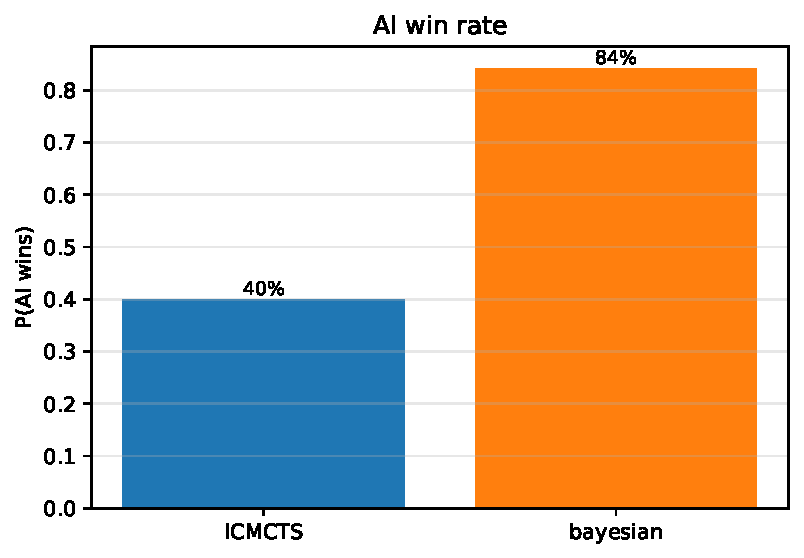
\includepdf[pages=-,pagecommand={\thispagestyle{plain}}]{games_analysis/ai_analysis_merged_players.pdf}

\section*{Mirror match (1{,}000)}
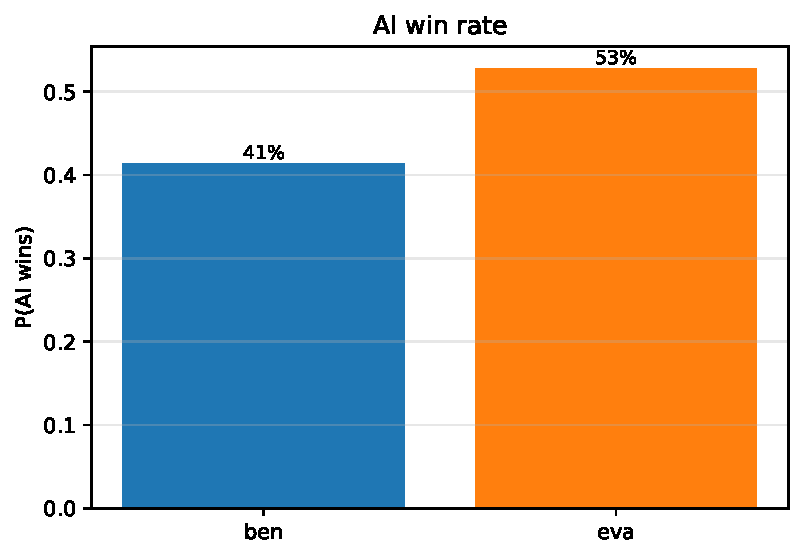
\includepdf[pages=-,pagecommand={\thispagestyle{plain}}]{games_analysis/ai_analysis_mirror.pdf}

\end{appendices}

\end{document}